% -*- Mode: LaTeX/P; fill-column: 80; -*-
% Local Variables:
% eval: (reftex-mode)
% eval: (TeX-PDF-mode)
% End:
% Template for PLoS
% Version 1.0 January 2009

% Whether to include the figures.
\newcommand*{\SHOWFIGS}{}%
\newcommand*{\SHOWDOC}{}%

\documentclass[10pt]{article}

% amsmath package, useful for mathematical formulas
\usepackage{amsmath}
% amssymb package, useful for mathematical symbols
\usepackage{amssymb}

% cite package, to clean up citations in the main text. Do not remove.
\usepackage{cite}

% Use doublespacing - comment out for single spacing
%\usepackage{setspace} 
%\doublespacing

% Text layout
\topmargin 0.0cm
\oddsidemargin 0.5cm
\evensidemargin 0.5cm
\textwidth 16cm 
\textheight 21cm

% Bold the 'Figure #' in the caption and separate it with a period
% Captions will be left justified
\usepackage[labelfont=bf,labelsep=period,justification=raggedright]{caption}

% Use the PLoS provided bibtex styles
\bibliographystyle{plos2009}

% Remove brackets from numbering in List of References
\makeatletter
\renewcommand{\@biblabel}[1]{\quad#1.}
\makeatother

% Leave date blank
\date{}

\pagestyle{myheadings}
%% ** EDIT HERE **
%% PLEASE INCLUDE ALL MACROS BELOW

\ifdefined\SHOWFIGS
% graphicx package, useful for including eps and pdf graphics
% include graphics with the command \includegraphics
\usepackage{graphicx}
\usepackage{color}
\usepackage{subcaption}
\pdfpagebox5
\usepackage{pgfplots}
\usepgfplotslibrary{dateplot}
\fi

\usepackage{tabularx}

\newcommand{\pop}{\textit{Populus spp.} }
\newcommand{\BLcond}{\ensuremath{BL_{cond}}}
\newcommand{\dbh}{\ensuremath{dbh}}
\newcommand{\DOB}{\ensuremath{DOB}}
\newcommand{\GIS}{\textsc{GIS}}
\newcommand{\LAIt}{\ensuremath{LAI_{T}}}
\newcommand{\LAI}{\ensuremath{LAI}}
\newcommand{\NPPdef}{\ensuremath{NPP_{def}}}
\newcommand{\NPPt}{\ensuremath{NPP_{T}}}
\newcommand{\NPP}{\ensuremath{NPP}}
\newcommand{\RP}{\ensuremath{RP}}
\newcommand{\Rdp}{\ensuremath{R_{\Delta\%}}}
\newcommand{\SLA}{\ensuremath{SLA}}
\newcommand{\SRWC}{\textsc{SRWC}}
\newcommand{\WF}{\ensuremath{W_F}}
\newcommand{\WS}{\ensuremath{W_S}}
\newcommand{\WR}{\ensuremath{W_R}}
\newcommand{\W}{\ensuremath{W}}
\newcommand{\dRres}{\ensuremath{\Delta R_{res}}}
\newcommand{\dW}{\ensuremath{\Delta W}}
\newcommand{\fAge}{\ensuremath{f_{age}}}
\newcommand{\fR}{\ensuremath{f_R}}
%\newcommand{\fi}{\ensuremath{f_i}}
\newcommand{\fT}{\ensuremath{f_T}}
\newcommand{\gbsm}{\textsc{GBSM}}
%\newcommand{\k}{\ensuremath{k}}
\newcommand{\lf}{\ensuremath{lf}}
\newcommand{\pRx}{\ensuremath{p_{R\%x}}}
\newcommand{\pfs}{\ensuremath{p_{FS}}}
\newcommand{\VI}{\ensuremath{VI}}
\newcommand{\sps}{\ensuremath{n_{stems}}}
\newcommand{\cancover}{\ensuremath{CanCover}}
\newcommand{\LA}{\ensuremath{LA}}

%% END MACROS SECTION

\begin{document}
\ifdefined\SHOWDOC
% Title must be 150 characters or less
\begin{flushleft}
{\Large
\textbf{Modeling Poplar Growth as a Short Rotation Woody Crop for Biofuels}
}
% Insert Author names, affiliations and corresponding author email.
\\
Q. J. Hart$^{1,\ast}$,
O. Prilepova$^{2}$,
J. R. Merz$^{1}$,
V. Bandaru$^{3}$
%N. C. Parker$^{3}$
B. M. Jenkins$^{4}$
\\
$^{\textbf{1}}$ Department of Land, Air, and Water, University of California, Davis, USA
$^{\textbf{2}}$ Department of Computer Science, University of California, Davis, USA
$^{\textbf{3}}$ Energy Institute, University of California, Davis, USA
$^{\textbf{4}}$ Department of Biological and Agricultural Engineering, University of California, Davis, USA
\\
%\\textbf{3} Author3 Dept/Program/Center, Institution Name, City, State, Country
$\ast$ E-mail: qjhart@ucdavis.edu
\end{flushleft}


% Please keep the abstract between 250 and 300 words
\section*{Abstract}

Short rotation woody crops (SRWC) such as hybrid poplar \pop are
potential feedstocks for cellulosic derived biofuels. The ability to accurately
predict the growth and biomass yields of SRWC under various environmental
conditions is important for predicting economic performance and overall
sustainability of the biofuel production system.  Tree coppicing is often used
in the management of SRWC plantations. Modeling the response of the SRWC to the
coppice cycle is a requirement in long term predictions of stand
productivity. The objective of this study was to develop a model of poplar
growth to evaluate feedstock supply potentials under different production
conditions including coppicing.  This was accomplished by modifying the
Physiological Principles in Predicting Growth (3PG) model originally developed
by Landsberg et al. (1997) to include a simple root interaction system to
simulate the sprouting and regrowth of coppiced trees. The modified model,
3PG-AHB, was tested against published information from three previous hybrid
poplar field studies employing coppicing.  Soil and weather inputs were
parameterized to be as close to the growing conditions as possible for the field
trials.  

The model parameterized with generic poplar derived values generally predicted
crop yield under coppicing to within the variations among different species
field tested.  The model's predictions were weakest in the first year after
coppicing events, improving thereafter. The model has been used as part of a
geospatial assessment of regional biomass production for the Pacific Northwest,
and appears to be useful for SRWC feedstock estimation.

\section*{Introduction}

Short rotation woody crops (SRWC) such as hybrid poplar (\textit{Populus spp.}),
willow (\textit{Salix spp.}), eucalyptus (\textit{Eucalyptus spp.}), and others have
been widely investigated as major bioenergy feedstocks for in the United States
and elsewhere.  (Perlack, 2005; Tuskan, 1998). SRWC culture has a number of
advantages including the potential for coppicing at harvest to allow for
regeneration of new plant growth without replanting (Hinchee et al., 2009; Aust
et al., 2013; Joslin and Schoenholtz, 1997; Sims and Venturi, 2004).

Cost-competitive biofuel development relies on a dependable supply of affordable
feedstock.  With purpose-grown crops such as SRWC as contrasted with wastes and
residues, the full cost of production is allocated to the feedstock and inputs
and yields are more critically important to the overall feasibility.  Biomass
production varies with spatial location, underlying soil properties, cultivation
practices, climate and management practices; hence, the ability to predict plant
biomass under different climate and management regimes is important to
developing management strategies that facilitate the best use of water, land,
fertilizers and other resources. For poplar and other SRWC, modeling the
physiological growth is advantageous because it allows for the variation of
species parameters and management practices in the presence of dynamic
environmental conditions. In addition, because the modeled canopy is carbon
balanced, allocations for both above and below ground biomass can be included in
lifecycle analyses of biofuel production in comparison to other fuel options
(reference). (reference).

Various models have been developed for SRWC simulation and applied with good
results (Gold and Seuring, 2011). One such model used for forest growth
simulations is the Physiological Principles in Predicting Growth (3PG)
model. The 3PG model has a simplified representation of biophysical processes
that control plant growth and requires limited input data (Landsberg et al.,
2003). As such, the model can easily be applied over large regions and for
multiple species with few modifications of the model parameters. Due to this
ease of application, 3PG has previously been used for modeling plant growth
within forests and plantations (Amichev et al., 2011). However, a missing from
prior implementations of 3PG for use with SRWC is a component addressing
coppicing and post-coppicing regrowth.

As part of the sustainability assessment under this initiative, we have extended
3PG to include coppicing by adding a component that allows for an additional
growth contribution from an existing root mass. The model specifies a relatively
small contribution to above-ground growth from the accumulated root mass after
coppicing in order to initiate the next cycle of production.  We parameterized
the model based on previously published results and compared the model results
to a set of field tests measuring poplar growth and yields in a coppiced regime.

% You may title this section "Methods" or "Models". 
% "Models" is not a valid title for PLoS ONE authors. However, PLoS ONE
% authors may use "Analysis" 
\section*{Methods}

\subsection*{Overview of the 3PG Model}

3PG is a forest carbon allocation model that is based on physiological
principles of using solar radiation for photosynthesis, primary production, and
the partitioning to the plant parts (i.e. foliage, stem, branches, bark and
roots) to determine the growth of the

plant~\cite{Landsberg1997,landsberg2010physiological}. 

The physiological
components of the original 3PG model comprises sub-modules for estimating growth
modifiers, Net Primary Productivity (NPP), biomass allocation, and soil water
balance (Figure~\ref{fig:growth-model}).  In general, the 3PG model works by
predicting expected productivity based on the soil, the current weather, and
their interaction with the species under consideration.  The model requires
input data in the form of 1) climate variables (maximum and minimum air
temperatures (°C), solar radiation (MJ m-2 day-1), rainfall (mm), vapor pressure
deficit (mbar) and number of frost days per month, 2) site and soil variables
including fertility, soil texture and water availability, 3) stand
initialization variables such as initial leaf, wood and root biomass and
allometric relationships, 4) management practices, for example, irrigation
scheduling, and 5) species information. At each time step, a potential maximum
value of productivity is calculated based on weather and climate conditions,
scaled by a number of multiplicative limiters derived from plant response to
temperature, water availability, fertility, and other species-dependent
processes.  The resulting productivity estimate is then allocated to the
different components of the plant.  At present the model uses a monthly time
step.

\subsection*{Poplar Hybrids parameterized for 3PG}

A few studies have specifically modeled poplar using the 3PG
model~\cite{Amichev2010,Headlee2012}. Headlee~\cite{Headlee2012} developed
Populus parameters from a set of both laboratory and field studies. These
parameters, with a few modifications, were used as the control set to
parameterize the growth of a representative hybrid poplar. As shown in
Section~\ref{sec:validation}, when compared to field trials the different
Populus clones vary considerably in their growth patterns. Many of these changes
can be modeled with appropriate changes to the 3PG input parameters
(Tables~\ref{tab:3pg-tree-productivity}, \ref{tab:3pg-tree-modifiers},
\ref{tab:3pg-tree-allocate}).

\subsection*{Coppicing Model}
\label{sec:coppicing-model}

The 3PG model allocates monthly productivity to the new roots, stems and
foliage. In the standard 3PG model, the amount of biomass allocated to the
foliage and stems is dependent on the age and size of the trees, while the
amount allocated to roots is essentially a constant allocation modified for
plant fertility stress. In SRWC, however, coppicing during harvesting results in
the stem and foliage being removed while the root ball remains. Because the
original model derives its production from transpiration, the original 3PG model
has no mechanism to start re-growth following coppicing due to the absence of a
foliar fraction.

Figure~\ref{fig:grow} shows the typical growth of a SRWC poplar tree.  Poplars
are generally propagated via cuttings of bare poplar stem inserted into
soil,~(Figure~\ref{fig:grow}a).  The cutting provides energy for the
establishment of the shoot and root buds~(Figure~\ref{fig:grow}b). As tree
matures, transpiration potsynthesis, and respiration provide for biomass
accumulation and growth.  This includes the establishment of the root
ball~(Figure~\ref{fig:grow}c).  By the time the poplar is ready for
coppicing~(Figure~\ref{fig:grow}d), the plants are well established.

After coppicing, resprouting occurs from the residual root and stem biomass
(Figure~\ref{fig:grow}e). In most species, multiple stems will sprout from the
same root and thinning may be necessary if single stems are required within the
SRWC harvest cycle although one shoot may eventually obtain dominance over
longer periods of time. (Figures~\ref{fig:grow}f
and~\ref{fig:grow}g). Modeling the growth of the SRWC then becomes, in part, a
task of determining the size and timing of the regrowth from the existing root
mass.

With no aerial shoot transpiration on which to initiate resprouting in the
original 3PG model, coppicing required the augmentation of the model to add this
capacity. This augmentation also allowed for model growth after the initial
planting of the cutting.

At any given time step, the model augments the productivity from the plant’s
transpiration with an additional production from utilization of reserves with in
the root mass. Under normal conditions, this augmentation is zero, however, with
the initial planting of the cutting, or after a coppicing event, this
augmentation is used to add foliage to the tree and restart transpiration-based
production.

The parameters of the model are shown in figure~\ref{fig:coppice}. Three species
specific parameters; Root Contribution (\Rdp), Leaf Area Index Target
(\LAIt), and Root Conversion Efficiency (\fR, control the coppicing
model. Combined with the input weather, and other parameters derived in the 3PG
model these control the extent and the timing of the regrowth from the coppiced
plant.

Only limited modifications are required to integrate the coppicing model into
the existing 3PG equations. At each monthly time step, the model allocates
productivity as before. The only difference is that total monthly growth (\dW) is
now the sum of the netp productivity (\NPP) and an additional root productivity
(\RP)~(Eq.\ref{eq:dw}). The contribution from \RP~however, is dependent on the weather, the state
of the plant, and parameters characterizing the root mass (Eq.~\ref{eq:rp}).

 \begin{align}
 \dW=\NPP+\RP \label{eq:dw} \\
 \RP = \begin{cases} 0 & \NPPdef <=0 \\
 \fR ~ min (\dRres ,\NPPdef) & \NPPdef > 0  
 \end{cases} \label{eq:rp}\\
 \NPPdef = \NPPt-\NPP \label{eq:nppdef}\\
 \dRres = \WR(\WR/\W - \pRx)\Rdp \label{eq:dRres}
 \end{align}

\RP~is affected by the potential of a plant to grow under the current weather
conditions as defined by the potential productivity of the plant. A target
productivity (\NPPt) within a given timestep can be defined from a target leaf
area index (\LAIt) that may or may not be realized in the current distribution of
biomass. The \LAIt~parameter can be thought of as defining a minimum \NPP~that the
plant is attempting to reach. an vary from 0 and greater. A zero value of \LAIt
indicates no root contribution, whereas positive values indicate contribution
from the roots simultaneous to \NPP~generated from foliage

Because the \NPPt~is affected by the current weather conditions, weather also
affects the root contribution. If conditions are not conducive to plant
transpiration, such as when cool, low sun conditions occur, then \NPPt~is low,
and resources are not allocated for growth. The deficit in (\NPPdef) is then
defined between the target \NPP~and the actual \NPP
(Eq.~\ref{eq:nppdef}). \NPPdef~defines a maximum contribution needed from the
roots to the overall plant growth to achieve the target productivity. The actual
contribution from the roots is limited by the amount of energy available in the
root mass at any given time.

The 3PG model includes a root allocation parameter, \pRx, that defines the root
size with respect to the total plant biomass. After coppicing, the root mass is
larger than the current value of \pRx~just before coppicing would specify. A
fraction of the extra root mass, \dRres~is available for production
(Eq.~(\ref{eq:dRres}). The parameter \Rdp~($0 ≤ \Rdp ≤ 1$) defines what fraction
of this surplus root mass can contribute to RP in a given time step. A value of
0 indicates no root contribution for regrowth while higher values indicate
increasing growth potential.

The root conversion efficiency, (\fR), ($0 ≤ \fR ≤ 1$) determines the mass of
new growth from the change in root mass andmultiplies the available root mass to
determine \RP.

In poplar plantations initially planted with cuttings, the original growth is
modeled in the same manner but using different values for \LAIt, \Rdp~and \fR.

Using climatic data for Corvallis, Oregon (Figure~\ref{fig:weather}), the
modified 3PG-AHB model was used to project biomass yields (Mg ha-1) with
coppicing occurring at different times (Figures~\ref{fig:date},~\ref{fig:rdp}
and~\ref{fig:lai}).

A plant parameterized with $\Rdp=1$, $\fR=1$ and $\LAIt=100$ will allocate
maximum resources into plant growth as fast as possible. This is an illustrative
example to show the effect of the season on the modeled regrowth.

Coppicing modeled in the third year in February, May, August, or November
(Figure~\ref{fig:date}) reveals that during periods with high potential
productivity (Feb-May), roots contribute more quickly to the regrowth of the
stem and foliage, matching the higher potential \NPP. Late season harvests defer
growth until the following spring conditions, and at a slower rate to match the
lower potential productivity at those times. The total production of the
plantation is affected by the timing of the coppicing suggesting an optimal
scheduling if model results accurately reflect actual growth, an objective of
model calibration and validation. For example, these model results give an
increase of 45\% yield over five years when coppicing in February vs. November
in the third year from planting.

Model predictions show the total foliage and root biomass converging to similar
values for all of the coppicing dates.

Root contribution (\Rdp) for coppicing in August and November during the third
year (Figure~\ref{fig:rdp}) shows a long term decrease in plant growth for very
low values of \Rdp~(0.001).  For but values of \Rdp~over about 0.1, the foliage
and stem growth are similar after the first 6 months of growth. While the root
contribution to productivity is smaller for lower values if \Rdp, the root
continues to contribute at each time step even while the root mass is small. The
root mass itself shows large differences over a longer period for these
variations in \Rdp. The productivity is closer for coppicing in November as the
potential productivities are smaller in the early months and the lower values of
\Rdp~still provide enough production given the environmental conditions. For
modeling actual trees, values of \Rdp~approaching 1 are unlikely as such high
values indicate mass that can readily be converted, primarily starches and
sugars. For poplar in particular, root starch and sugar contents vary with the
root diameter ranging up to as much as 20\% of total root mass. A value of
$\Rdp=0.1$ is used for the validations against field trials described below.

Changes in \LAIt~from 0.1 to 10 (Figure~\ref{fig:lai}) for the same August and
November coppicing events in the third year with \Rdp~set to 0.1 yield up to
10\% change in total stem biomass production over five years for the later
harvest. There is little dependence on \LAIt~for values greater than about 1.

\LAI~is chosen as the primary target parameter for the 3PG model as it is a
simple plant parameter controlling productivity. Its primary effect at a given
time step is to affect the light gathering capacity of the tree. That fraction
is given in the 3PG model as $1−\exp{-k LAI}$. For poplar, we have defined $k =
0.5$ and the productivity of the tree starts to become dominated by this value
with relatively low values of \LAI.  Final values of the coppicing parameters
selected for use with the modified 3PG model vary slightly between the cutting
at planting and the subsequently coppiced trees
(Table~\ref{tab:3pg-tree-coppice}).

\section*{Results and Discussion}
\label{sec:validation}

The 3PG model was tested against results from three published field studies of
coppiced \pop [\cite{Proe2002,Proe1999,Pontailler1999,Afas2008a}]. We chose
field tests that included at least one coppicing rotation, measurements of
above-ground biomass, and enough information to simulate plant growth and
biomass yields with some level of confidence. Along with above ground biomass,
additional parameters reported by each field study were compared with the model
results when possible.  These parameters include allometric relationships for
biomass partitioning, ratios of above-ground to root biomass, and additional
measurments such as Leaf Are Index, \LAI.

In each case, input weather conditions were obtained for the time of the field
work, and management practices and soil parameters were either obtained or
estimated from the description in the literature (Table~\ref{tab:field-test-manage}).

The primary comparision was of model preditions to measured values for woody
biomass.  Twenty-one measured values were included.  A generic set of parameters
for poplar were used.  However, as described in Section~\ref{sec:pont}, two
methods for determing the partioning ratios of foilage to woody biomass were
included.  The number of coppice events ranged from 0 to 5, and the age of the
tree for a coppice cylce ranged from 0.3 to 5.3 years.  Two studies included
multiple poplar clones in the field tests (Table~\ref{tab:field-summary}).

\subsection*{Field Trial 1 - Pontailler 1999}
\label{sec:pont}

Pontailler~\cite{Pontailler1999,pontailler97-volume-index,Ceulemans1993},
described the results of biomass measurements over 5 two year coppicing events
for a five different poplar species, grown in Orsay, France from 1987 through
1997. Poplar clones studied included fast growing, interspecific Interamerican
(\textit{Populus trichocarpa $\times$ P deltoides}) hybrid clones (Beaupré and
Raspalje), a native American \textit{P. trichocarpa} clone (Fritzi Pauley) and
one Euramerican reference clone \textit{P.~deltoides $\times$ P.~nigra}, cv.,
(Robusta).

All were planted from cuttings. At each coppicing event, woody biomass yields,
stem diameter, tree height, number of stems per stump and LAI were among the
parameters measured.  Weather data were obtained for Orsay during the same
period of time from the Tutiempo Network~\cite{Geiger2002,TutiempoNetwork2013}
(Figure~\ref{fig:pontailler-weather}).

For the most part this field study reported consistently high biomass. It was
reported that the first two coppicing cycles the plantations included some
fertilization and irrigation, but applications stopped after the second
coppice. These affect the 3PG fertility and water availability inputs.  There
were variations in yields for the final three coppicing events and these
differences, especially the lower yields in 1991-1992, were attributed to
drought conditions for the region.

Comparisons with 3PG-AHB model predictions (Figure~\ref{fig:pont-biomass}) show
that the model described above under-predicts most yield data results
obtained.by Pontailler, et al.  For this field test, the differences are most
likely due to different management practices as compared to implicit assumptions
of the control model. Two of the most important considerations are the high
density of plantings and the frequency of coppicing, both of which affect model
assumptions.  In particular, the allocation of the biomass among the roots,
stems, and foilage.

An important component of 3PG is the allocations of \NPP~to roots, stems, and
foliage.  This is controlled primarily with the \pfs, the ratio of \WF~to \WS,
$\pfs=\WF/\WS$, which helps determine the aboveground allocations.  \pfs~is in
turn calculated from a pair of allometric relations.  In 3PG, \pfs~is obtained
in a two step process, first obtaining an estimate of \dbh~from the current \WS,
and then using \dbh~to determine \pfs~through a measured relationship.  These
relations are typically determined from comparisons of more mature trees, for
example, Headlee's estimates are based on poplars with a range in \dbh~of about
3.5~-~25 (cm)~\cite{Headlee2012}%,Fortier2010}.

For frequent coppicing with small trees at harvest, an alternative set of
allometric relationships to determine \pfs~for the 3PG might be required. For
SRWC, Pontailler et al.~\cite{pontailler97-volume-index} proposed a set of
parameterizations based on volume index (\VI) where $VI = HD^2$, $H$ is height
(m), and $D$ is tree diameter (m) at 22cm.

Pontailler et al.~\cite{pontailler97-volume-index} described power relationships
between \VI~and both above ground dry matter and leaf area per stem. These can
be used in a similar manner to define \pfs, where \WS~is inverted to estimate
\VI~for each stem, and then used to predict leaf area per stem (\LA) and along
with specific leaf area (\SLA), \WF~and \pfs. As these relationships were
defined for each poplar variation in the field tests, the 3PG model was modified
to predict \pfs~with these relationships, and the model run with the parameters
shown in Table~\ref{tab:pont-3pg}.  Because of the high density of tree
plantings, the canopy coverage (\cancover), which determines when the poplar
canopy has closed was scaled from 1.5 years post-coppicing to 0.6 yrs
(Figure~\ref{fig:pont-biomass}). The poplar stem biomass demonstrates a wide
variation under the same management practices. However, without more information
relating to the various \pop clones, modifying 3PG parameters to obtain a better
fit is mostly speculative. The 3PG inputs can be adjusted to more closely match
the predictions for each clone, but justifying which particular parameters to
adjust from one field test is more problematic and the selection essentially
arbitrary.

To illustrate, the variation of one poplar clone, Raspalje, is demonstrated over
a few of the more important 3PG inputs (Figure~\ref{fig:pont-variation}). The
quantum efficiency directly affects the monthly NPP. Although this is constant
in the 3PG model, lab measurements show clonal and seasonal variations of up to
0.02 mol C/mol PAR, usually with maxima in the region of 0.08 mol C/mol
PAR~\cite{Bernacchi2003}.

Other interesting observations relate to the variations from year to
year. Certain 3PG parameters, such as growth modifiers that are dependent on
temperature or the available soil water should show dependence on the input
weather parameters. Matching this inter-coppicing variability would lend some
justification for modification of those parameters.

Model stem yield is also influenced by the optimal temperature and maximum tree
conductance (Figure~\ref{fig:pont-variation}). Neither can account for the
changes in the field trials, especially the dip in 1992-1993, or the peak in the
following coppice cycle. The tree canopy conductance shows a small variation
with a shape somewhat more weather dependent, but not at the scale shown in the
trials.  The general downward trend in yield over the last three coppicing
cycles is due to poor weather.  The weather estimates from the data obtained for
the model may not have adequately represented variations during the field trial.

The 3PG model includes a tree aging limiter, parameterized in part by the age
whhere the limitation is one half.  This is the primary modifier affecting
decreased productivity of multiple copping cycles.

The 3PG model uses a linear relation with the stand age to determine canopy
cover, which also linearly affects the \NPP~for each month. In the
parameterization of the poplar trees, Headlee et al.\cite{Headlee2012} used
canopy cover as a variable to match the observed yields of some of the field
tests. However, on a highly dense plantation, the canopy might close more
quickly, resulting in higher productivity in the months after a coppicing event.

As an exercise, the 3PG inputs were modified for each poplar type, to determine
if the overall shapes of the measured growth could be replicated by some
parameterization of the model.  These results are shown in
Figure~\ref{fig:pont-best}.  Some of the inputs shown in
Figure~\ref{fig:pont-variation} were modified independantly for each
type. Without independant verification of the input values used, using
parameters obtained with such a method are fairly speculative.

\subsection*{Field Trial 2 - Proe et al. 2002}

Proe et al.~\cite{Proe2002} described the results of different \SRWC~field
trials, including annual measurements of biomass, root:shoot ratio, leaf/stem
ratios, \LAI~and other parameters. The studies were developed over a 5 year
period in central Scotland from 1989 through 1999. For the coppicing study,
balsam spire poplars (\textit{Populus balsamifera} var. \textit{Michauxii}
(Henry) $\times$ \textit{Populus trichocarpa} var. \textit{Hastata} (Dode)
Farwell) were planted at uniform 1 (m) spacing.  However, there was only one
coppicing event in the first year for comparison. Proe et al. destructively
tested plantation samples over the course of the growing cycle.  The field test
of Proe et al. differs from the previous field study by Pontailler et al. in
having a longer coppicing cycle, additional measurements within a cycle, and
alternative data collected, in particular the ratios of the various fractional
constituents of the poplar plants.  Comparisons with the 3PG model were made by
simulating the plantings under the conditions described. Weather information
(Figure~\ref{fig:proe-weather}) for the Scotland field plots was obtained for
Paisley, Scotland~\cite{Proe2002,MetOffice2013}. Calculated clear sky radiation
was moderated by the ratio of observed daylight hours to total
daylight. Comparisons of woody biomass, \LAI, and fraction of foliage to above
ground biomass were made between the 3PG model and the measured values for
single stem and coppiced practices.  In addition, two different allometric
relations were used, the dbh version from Headlee et al.\cite{Headlee2012} and a
representative \VI~relation (raspalje) from the Pontailler study,
(Figure~\ref{fig:proe-wood}). 

The additional measurements in the Proe et al. study, hightlight the affects
that differences in the allometric relationships have on the predictions.  The
\VI~relation based methods seems to track the foilage estimations better, while
the \dbh~relation tracks stem biomass slightly better.  Both models are over
predicting the total biomass, with the partitioning affecting the measurment
comparisons.  The fact the that the \VI~model tracks $frac{WF}{WF+WS}$ fairly
well, but not \LAI~for the coppiced model indicates that the modeled form of
\LAI~is not asor possibly a different \SLA~parameter for these poplar
trees. Proe also noted low values of \LAI~were related to insect damage,
especially in the third and fourth years. Proe independently showed the canopy
to close in about 16 months from initial planting for both trials, which is
considerably longer than the model paremeter of 6 months for full canopy
closure.

Because Proe et. al include root:shoot ratios, an overprediction of root biomass
is indicated.  Though not shown, modifications to the root allocation
parameters, can model these measured values.  These changes possibly due to the
very wet nature of the field trial soil.

\subsection*{Field Trial 3 - (Afas 2008)}
\label{afas2008}

Starting in 1996, Afas,~\cite{Afas2008a} studied multiple poplar clones over the
course of 11 years for a field study in Belgium~\cite{Laureysens2005,Laureysens2004}.
The study included measurements of three separate coppicing events.  The study
found relatively high mortality rates for some of the genotypes.  Comparisons
between the 3PG and measured values were made for the genotypes with a survival
rate of over 85\%.  No measurements of below ground biomass were included.  Afas
did propose an allometric relationship for non-destructive biomass estimations
based on diameter measurements of the stems from the stool, but for consistency,
the allometric relations identified in the Pontailler et. al study were used in
the model comparisons.  Based on the field description, plant densities were
determined, and soil conditions estimated (Table~\ref{tab:field-test-manage}).

These results are similar to the Pontailler study, with a fairly large
distribution among the varieties, but differ in that the model in this case does
not follow the measurement patterns in the same way.  The first noticable
difference is the model generally overpredicts the final woody biomass
measurements, immediately preceeding the coppicing events, although the \dbh~
based estimates are within the envelope of the clones.  At the same time, the
intermediate comparisons often show the model underpredicting the measured
values, especially in the earliest post-coppicing measurements.  As with the
Pontailler study, individual parameterizations of the 3PG model would result in
better fitting, (Section~\ref{sec:pont}),
(Figures~\ref{fig:pont-variation}~and~\ref{fig:pont-variation}), with the same
considerations.  One consideration, however, is that the plant configuration
choosen for this study, using alternating inter-row distanes and closer row
spacings, positively affects the canopy closure for this plantation.  This would
show increased productivity in the earlier stages of growth after coppicing.
The fact that this isn't a consistent trend in the 2nd and 3rd cycles would be
harder to capture in the model.

\section*{Conclusions}

The model introduced in this paper to add coppicing events to the 3PG
application seems to behave adequatel.  In fact, parameter variation suggest
that the modified 3PG model is somewhat insensitive to the parameters when
chosen in reasonable bounds. We have used this coppicing model in the validation
section above to predict poplar regrowth in multi-coppicing scenarios.  However,
when comparing the model to field validation, the published studies focus on
yields over complete coppicing cycles or at least at yearly timesteps.
Observations to test the model in those important months directly after a
coppice, or under a more complete range of coppicing event types are lacking for
comparision.

Although not considered in current model, there are other considerations when
coppicing during the growing season.  Also, the current model defines a constant
value for \Rdp. Studies of the available starches and sugars in a poplar root
suggest a seasonal dependence on these values, with higher values as the plants
enter into cooler seasons~\cite{Regier2010}. The field trials above all coppiced
at the end of the growing season, but these are important considerations when
considering other strategies, like store on stump management for more continuous
feedstock delivery.  The 3PG model includes a stump mortality component, but not
one based on coppicing, and that was not included in these studies.  However,
Afas in particular identified high rates of tree mortality, and the tree
mortality estimations, especially in the context of coppicing events can be
revisited.
%some studies have identified higher rates of stump
%depth related to coppicing in the growing season~\cite{}.

Validation of the model with respect to previously published field trials of
poplar for a number of different locations and management strategies, led to a
number of conclusions, regarding poplar growth. First, the differences among
clones in terms of the productions and yields are often quite large. A
generalized model is only an estimate on behavior. The model discussed here
comes in somewhere in the middle of the field trials investigated.

For high density plantations of \SRWC~with higher coppicing cycles, using
allometric relations based on a parameter like the Volume Index (\VI) as opposed
to the \dbh~is probably preferable. It should be noted however, that these
relationships are also possibly dependent on the planting density, and care
should be used when applying under different management scenarios. These
relationships seem to vary with the duration of the coppicing cycle  as well.  

For \SRWC~the relationships between canopy cover, plantation density, and stems
per stump resprouting could be investigated to determine some repeatable
relationships between this parameters that could be added into the 3PG model as
well.

In general it can be a difficuly task to identify what parameters can be
reasonably varied in the 3PG when attempting to understand the differences in
growth between clonal varieties.  Section~\ref{sec:pont} included some
discussion for this task.  However, multiple parameters can effect the growth in
the same way.  This is especially true for consistent bias between the model and
measurements, where many parameters can uniformly decrease or increase the
amount of potential productivity that is captured for plant growth.


% Do NOT remove this, even if you are not including acknowledgments
\section*{Acknowledgments}
This work is supported by an Agriculture and Food Research Initiative
Competitive Grant no. 2011-68005-30407 from the USDA National Institute of Food
and Agriculture (NIFA).

%\section*{References}
% The bibtex filename
\bibliography{ahb-pnw}

\newpage
\section*{Figure Legends}
\fi

\begin{figure}%[p]
\ifdefined\SHOWFIGS
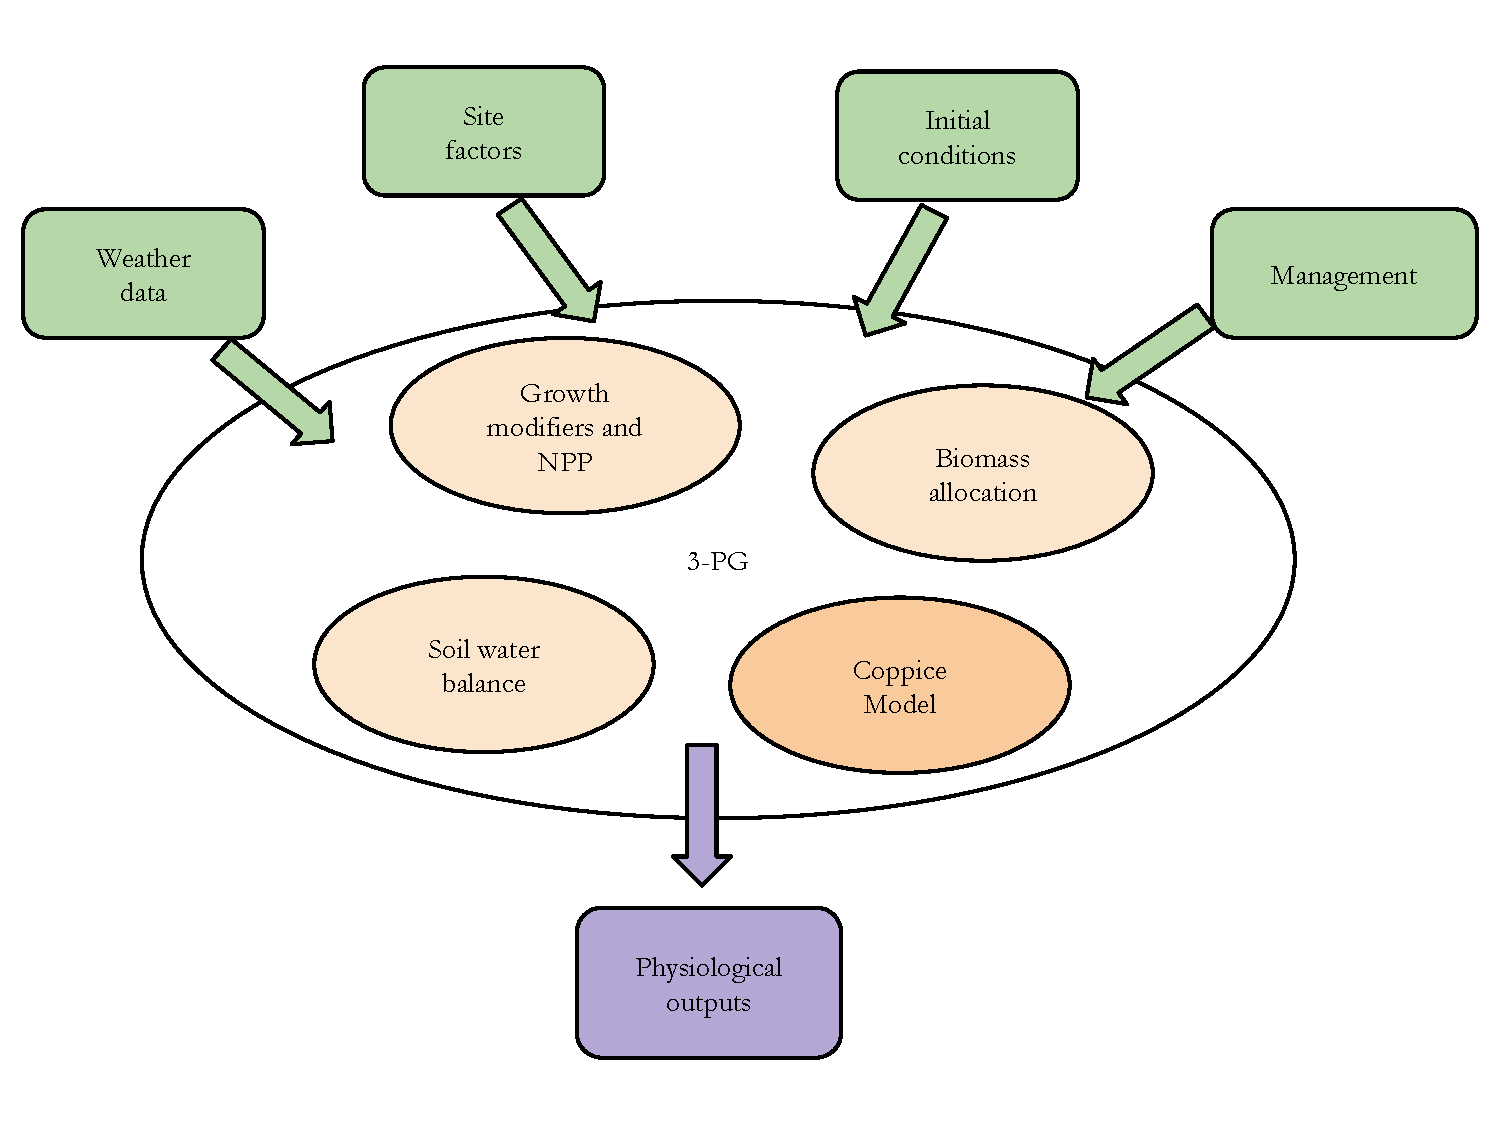
\includegraphics[width=\linewidth]{model_overview}
\fi
\caption{ { \bf 3PG Overview. } }
\label{fig:growth-model}
\end{figure}

\begin{figure}%[p]
\ifdefined\SHOWFIGS
\begin{subfigure}[b]{.1125\linewidth}
\centering
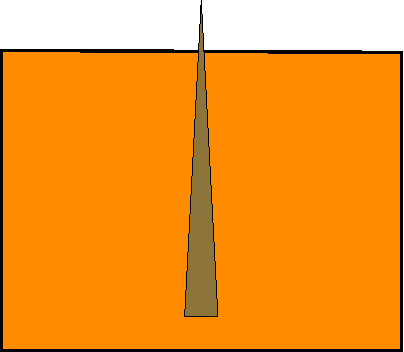
\includegraphics[width=1.0\linewidth]{img/tree_pics_1}
\caption{}  %\caption{planting}
\label{fig:grow_1}
\end{subfigure}
\begin{subfigure}[b]{.1125\linewidth}
\centering
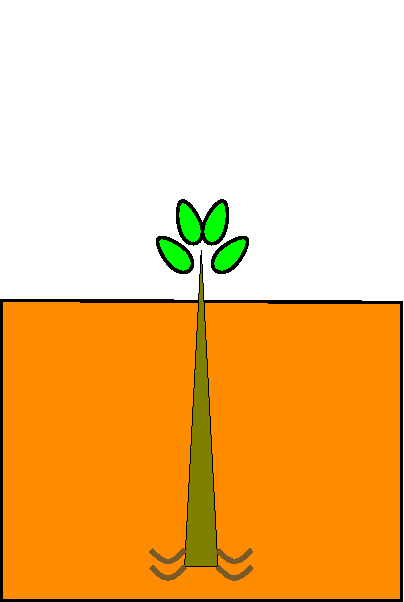
\includegraphics[width=1.0\linewidth]{img/tree_pics_2}
\caption{}  %\caption{sprout}
\label{fig:grow_2}
\end{subfigure}
\begin{subfigure}[b]{.1125\linewidth}
\centering
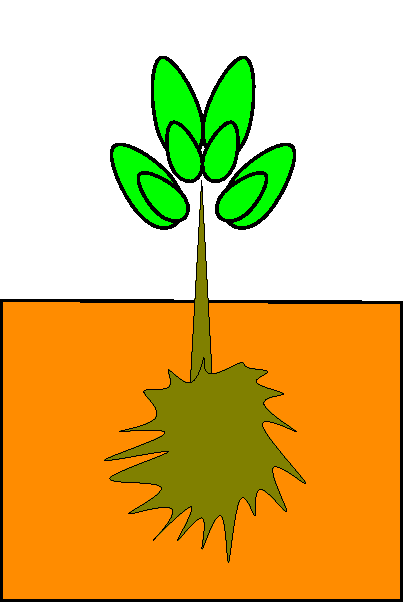
\includegraphics[width=1.0\linewidth]{img/tree_pics_3}
\caption{}  %\caption{growth}
\label{fig:grow_3}
\end{subfigure}
\begin{subfigure}[b]{.1125\linewidth}
\centering
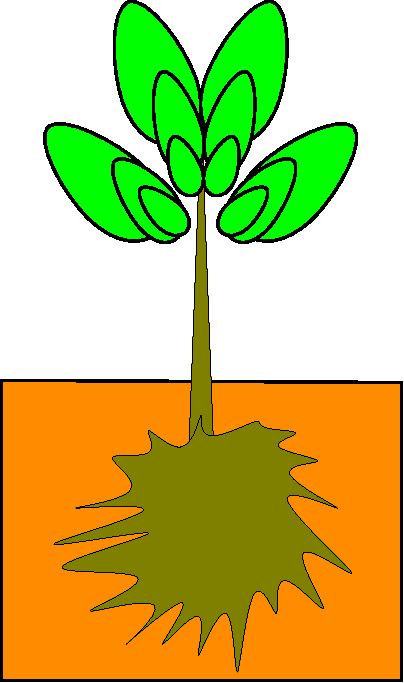
\includegraphics[width=1.0\linewidth]{img/tree_pics_4}
\caption{}  %\caption{maturity}
\label{fig:grow_4}
\end{subfigure}
\begin{subfigure}[b]{.1125\linewidth}
\centering
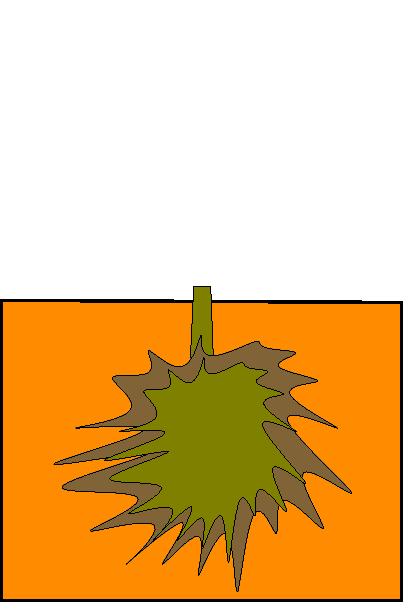
\includegraphics[width=1.0\linewidth]{img/tree_pics_5}
\caption{}  %\caption{coppiced}
\label{fig:grow_5}
\end{subfigure}
\begin{subfigure}[b]{.1125\linewidth}
\centering
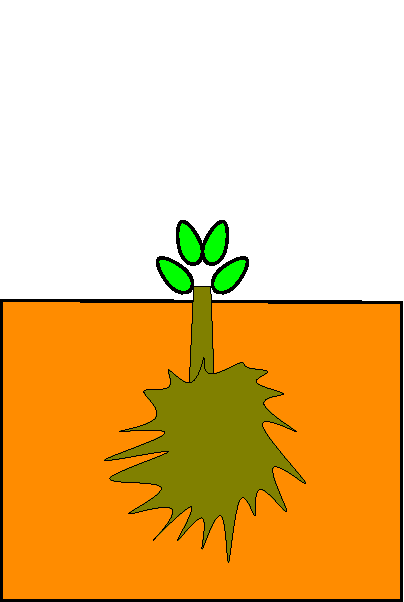
\includegraphics[width=1.0\linewidth]{img/tree_pics_6}
\caption{}  %\caption{resprouting}
\label{fig:grow_6}
\end{subfigure}
\begin{subfigure}[b]{.1125\linewidth}
\centering
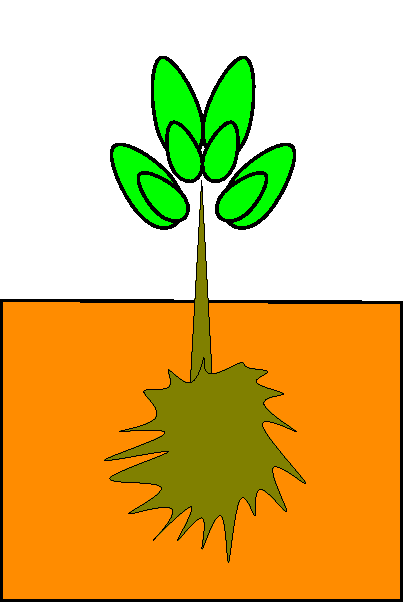
\includegraphics[width=1.0\linewidth]{img/tree_pics_7}
\caption{}  %\caption{regrowth}
\label{fig:grow_7}
\end{subfigure}
\begin{subfigure}[b]{.1125\linewidth}
\centering
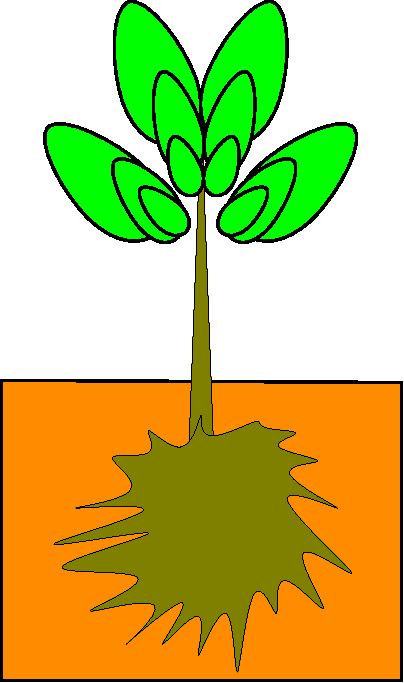
\includegraphics[width=1.0\linewidth]{img/tree_pics_4}
\caption{}  %\caption{next harvest}
\label{fig:grow_8}
\end{subfigure}
\fi
\caption{ {\bf Poplar \SRWC~growth.} The growth stages for poplar
  grown as an \SRWC~with one coppicing cycle shown. }
\label{fig:grow}
\end{figure}

\begin{figure}%[p]
\ifdefined\SHOWFIGS
   \centering
% \begin{subfigure}[b]{.2\linewidth}
   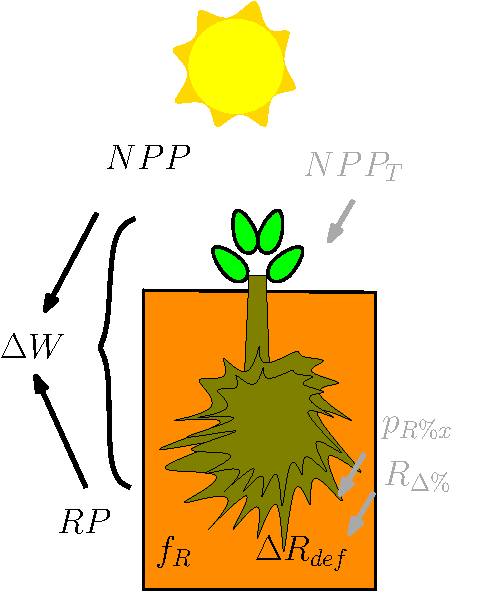
\includegraphics[width=0.3\linewidth]{img/tree_pics_10}
 %  \caption{Parameters}
 %  \label{fig:coppice-img}
% \end{subfigure}
% \quad
% \begin{subtable}[b]{.75\linewidth}
% \begin{align}
% \dW=\NPP+\RP \\
% \RP = \begin{cases} 0 & \NPPdef <=0 \\
% \fR ~ min (\dRres ,\NPPdef) & \NPPdef > 0  
% \end{cases} \\
% \NPPdef = \NPPt-\NPP \\
% \dRres = \WR(\WR/\W - \pRx)\Rdp
% \end{align}
% \caption{}
% %\caption{Model Definition}
% \end{subtable}
\fi
\caption{ {\bf Coppice Model Overview.} }
\label{fig:coppice}
\end{figure}

\begin{figure}%[p]
\ifdefined\SHOWFIGS
  \centering
  \definecolor{color1}{HTML}{3366CC}
\definecolor{color2}{HTML}{DC3912}
\definecolor{color3}{HTML}{FF9900}
\definecolor{color4}{HTML}{109618}
\definecolor{color5}{HTML}{990099}
\definecolor{color6}{HTML}{0099C6}


\begin{tikzpicture}
  \begin{axis}[
    no markers,
    width=0.8\linewidth,
    height=2in,
    %date coordinates in=x,
    %xticklabel={\month},
    ylabel style={align=center}, ylabel=Rad {$[MJ/day]$}; Temp {$[C]$}\\ Daylight {$[hr]$},
    xlabel style={align=center}, xlabel=Month,
    %stack plots=false,
    xmin=.8,
    xmax=12.2,
    bar width=3pt,
    legend entries={$T_n$,$T_x$,$R$,$Hrs$},
    legend style={at={(0.4,1.03)},anchor=south},
    legend columns=4,
    %legend to name = temp
    % legend style={
    % at={(0.5,-0.3)},anchor=north,legend columns=-1}
    ]
    \addplot+[color=color1,line width=1pt] table [x=month, y=tmin, col sep=comma] {coppice/weather.csv};
    \addplot+[color=color2,line width=1pt] table [x=month, y=tmax, col sep=comma] {coppice/weather.csv};
    \addplot+[ybar, ybar legend, color=color5, fill=color5] table [x=month, y=rad, col sep=comma] {coppice/weather.csv};
    \addplot+[ybar, ybar legend, bar shift=4pt, color=color6, fill=color6] table [x=month, y=daylight, col sep=comma] {coppice/weather.csv};
    
  \end{axis}
  \begin{axis}[
     no markers,
     width=0.8\linewidth,
     height=2in,
     xmin=.8,
     xmax=12.2,
  %   date coordinates in=x,
  %   ylabel=PPT [mm],
     axis y line=right,
     axis x line=none,
  %   % ylabel style={yshift=10pt},
     legend entries={$PPT$},
     legend style={
        at={(.7,1.03)},
        anchor=south},
     %legend to name = ppt,
     ylabel style={align=center}, ylabel=Precip {$[mm]$},
     ]
    \addplot+[color=color4,line width=1pt] table [x=month, y=ppt, col sep=comma] {coppice/weather.csv};
   \end{axis}
\end{tikzpicture}
%\ref{temp}

\fi
  \caption{ {\bf Illustrative weather data.} Weather parameters replicating
    conditions similar to those found in Corvallis, OR}
  \label{fig:weather}
\end{figure}

\begin{figure}%[p]
\ifdefined\SHOWFIGS
  \centering
  \pgfplotsset{
      no markers,
      width=\linewidth,
      height=0.25\linewidth,
      every axis plot/.append style={line width=1pt},
      date coordinates in=x,
      xmin={2016-02-15},
      xmax={2019-10-15},
      xtick={2016-06-15,2016-09-15,2016-12-15,
      2017-03-15,2017-06-15,2017-09-15,2017-12-15,
      2018-03-15,2018-06-15,2018-09-15,2018-12-15,
      2019-03-15,2019-06-15,2019-09-15},
      x tick label style={rotate=45, anchor=east},
      xticklabels={Y2-06,Y2-09,Y2-12,
      Y3-03,Y3-06,Y3-09,Y3-12,
      Y4-03,Y4-06,Y4-09,Y4-12,
      Y5-03,Y5-06,Y5-09},
      ymin=0,ymax=60,
      ytick={20,40},
      yticklabels={20,40},
}
  \begin{tikzpicture}
    \begin{axis}[
      name=feb,
      legend entries={Stem,Root,Foilage},
      legend style={
        at={(0.5,1)},anchor=south,legend columns=-1,yshift=1pt},
      xticklabels=\empty,
      ]
      \node[right] at (axis cs:{2016-02-15},50) {Y3-02};
      \addplot+[color=brown] table [x=date, y=m02f1, col sep=comma] {coppice/hart12coppice-coppice-ws.csv};
      \addplot+[color=red] table [x=date, y=m02f1, col sep=comma] {coppice/hart12coppice-coppice-wr.csv};
      \addplot+[color=green] table [x=date, y=m02f1, col sep=comma] {coppice/hart12coppice-coppice-wf.csv};
    \end{axis}
    \begin{axis}[
      name=may,
      at={(feb.below south west)},yshift=5pt,
      anchor=north west,
      xticklabels=\empty,
      ]
      \node[right] at (axis cs:{2016-02-15},50) {Y3-05};
      \addplot+[color=brown] table [x=date, y=m05f1, col sep=comma] {coppice/hart12coppice-coppice-ws.csv};
      \addplot+[color=red] table [x=date, y=m05f1, col sep=comma] {coppice/hart12coppice-coppice-wr.csv};
      \addplot+[color=green] table [x=date, y=m05f1, col sep=comma] {coppice/hart12coppice-coppice-wf.csv};
    \end{axis}
    \begin{axis}[
      name=aug,
      at={(may.below south west)},yshift=5pt,
      anchor=north west,
      xticklabels=\empty,
      ]
      \node[right] at (axis cs:{2016-02-15},50) {Y3-08};
      \addplot+[color=brown] table [x=date, y=m08f1, col sep=comma] {coppice/hart12coppice-coppice-ws.csv};
      \addplot+[color=red] table [x=date, y=m08f1, col sep=comma] {coppice/hart12coppice-coppice-wr.csv};
      \addplot+[color=green] table [x=date, y=m08f1, col sep=comma] {coppice/hart12coppice-coppice-wf.csv};
    \end{axis}
    \begin{axis}[
      name=nov,
      at={(aug.below south west)},yshift=5pt,
      anchor=north west,
      height=0.2916\linewidth,
      ymin=0,ymax=70,
      ytick={20,40,60},
      yticklabels={20,40,60},
      ]
      \node[right] at (axis cs:{2016-02-15},50) {Y3-11};
      \addplot+[color=brown] table [x=date, y=m11f1, col sep=comma] {coppice/hart12coppice-coppice-ws.csv};
      \addplot+[color=red] table [x=date, y=m11f1, col sep=comma] {coppice/hart12coppice-coppice-wr.csv};
      \addplot+[color=green] table [x=date, y=m11f1, col sep=comma] {coppice/hart12coppice-coppice-wf.csv};
    \end{axis}
  \end{tikzpicture}

\fi
  \caption{{\bf Coppice regrowth model results.}  Results for various coppicing
    dates.  Y-axis is the dry mass of each component of the plantation, in terms
    of $\frac{T}{ha}$.}
  \label{fig:date}
\end{figure}

\begin{figure}%[p]
\ifdefined\SHOWFIGS
  \centering
  \pgfplotsset{
      no markers,
      width=0.5\linewidth,
      height=0.25\linewidth,
      every axis plot/.append style={line width=1pt},
      date coordinates in=x,
      xmin={2017-03-15},
      xmax={2019-10-15},
      xtick={
      2017-06-15,2017-09-15,2017-12-15,
      2018-03-15,2018-06-15,2018-09-15,2018-12-15,
      2019-03-15,2019-06-15,2019-09-15},
      xticklabels=\empty,
}
  \begin{tikzpicture}
    \begin{axis}[
      name=ws08,
      ymin=0,ymax=80,
      ytick={20,40,60},
      yticklabels={20,40,60},
      ylabel=Stem~$\frac{T}{ha}$,
      legend entries={$\Rdp=0.001$,$\Rdp=0.01$,$\Rdp=0.1$,$\Rdp=0.5$,$\Rdp=1$},
      legend style={
        at={(1.0,1.0)},anchor=south,legend columns=-1,yshift=2pt}
      ]
      \node[right] at (axis cs:{2018-02-15},50) {Aug};
      \addplot+[color=red] table [x=date, y=m08f0.001, col sep=comma] {coppice/hart12coppice-coppice-ws.csv};
      \addplot+[color=orange] table [x=date, y=m08f0.01, col sep=comma] {coppice/hart12coppice-coppice-ws.csv};
      \addplot+[color=yellow] table [x=date, y=m08f0.1, col sep=comma] {coppice/hart12coppice-coppice-ws.csv};
      \addplot+[color=green] table [x=date, y=m08f0.5, col sep=comma] {coppice/hart12coppice-coppice-ws.csv};
      \addplot+[color=blue] table [x=date, y=m08f1, col sep=comma] {coppice/hart12coppice-coppice-ws.csv};
    \end{axis}
    \begin{axis}[
      name=ws11,
      at={(ws08.east)},xshift=2pt,
      anchor=west,
      ymin=0,ymax=80,
      ytick={20,40,60},
      yticklabels=\empty
      ]
      \node at (axis cs:{2018-02-15},50) {Nov};
      \addplot+[color=red] table [x=date, y=m11f0.001, col sep=comma] {coppice/hart12coppice-coppice-ws.csv};
      \addplot+[color=orange] table [x=date, y=m11f0.01, col sep=comma] {coppice/hart12coppice-coppice-ws.csv};
      \addplot+[color=yellow] table [x=date, y=m11f0.1, col sep=comma] {coppice/hart12coppice-coppice-ws.csv};
      \addplot+[color=green] table [x=date, y=m11f0.5, col sep=comma] {coppice/hart12coppice-coppice-ws.csv};
      \addplot+[color=blue] table [x=date, y=m11f1, col sep=comma] {coppice/hart12coppice-coppice-ws.csv};
    \end{axis}

    \begin{axis}[
      name=wf08,
      ylabel=Foilage,
      at={(ws08.below south west)},yshift=5pt,
      anchor=north west,
      ymin=0,ymax=30,
      ytick={10,20},
      yticklabels={10,20},
      ]
%      \node[right] at (axis cs:{2016-02-15},50) {Aug};
      \addplot+[color=red] table [x=date, y=m08f0.001, col sep=comma] {coppice/hart12coppice-coppice-wf.csv};
      \addplot+[color=orange] table [x=date, y=m08f0.01, col sep=comma] {coppice/hart12coppice-coppice-wf.csv};
      \addplot+[color=yellow] table [x=date, y=m08f0.1, col sep=comma] {coppice/hart12coppice-coppice-wf.csv};
      \addplot+[color=green] table [x=date, y=m08f0.5, col sep=comma] {coppice/hart12coppice-coppice-wf.csv};
      \addplot+[color=blue] table [x=date, y=m08f1, col sep=comma] {coppice/hart12coppice-coppice-wf.csv};
    \end{axis}

    \begin{axis}[
      name=wf11,
      at={(wf08.east)},xshift=2pt,
      anchor=west,
      ymin=0,ymax=30,
      ytick={10,20},
      yticklabels=\empty
      ]
%      \node[right] at (axis cs:{2016-02-15},50) {Nov};
      \addplot+[color=red] table [x=date, y=m11f0.001, col sep=comma] {coppice/hart12coppice-coppice-wf.csv};
      \addplot+[color=orange] table [x=date, y=m11f0.01, col sep=comma] {coppice/hart12coppice-coppice-wf.csv};
      \addplot+[color=yellow] table [x=date, y=m11f0.1, col sep=comma] {coppice/hart12coppice-coppice-wf.csv};
      \addplot+[color=green] table [x=date, y=m11f0.5, col sep=comma] {coppice/hart12coppice-coppice-wf.csv};
      \addplot+[color=blue] table [x=date, y=m11f1, col sep=comma] {coppice/hart12coppice-coppice-wf.csv};
    \end{axis}

    \begin{axis}[
      name=wr08,
      at={(wf08.below south west)},yshift=5pt,
      anchor=north west,
      x tick label style={rotate=45, anchor=east},
      xticklabels={
      Y3-06,Y3-09,Y3-12,
      Y4-03,Y4-06,Y4-09,Y4-12,
      Y5-03,Y5-06,Y5-09},
      ymin=5,ymax=30,
      ytick={10,20},
      yticklabels={10,20},
      ylabel=Root,
      ]
%      \node[right] at (axis cs:{2016-02-15},30) {Aug};
      \addplot+[color=red] table [x=date, y=m08f0.001, col sep=comma] {coppice/hart12coppice-coppice-wr.csv};
      \addplot+[color=orange] table [x=date, y=m08f0.01, col sep=comma] {coppice/hart12coppice-coppice-wr.csv};
      \addplot+[color=yellow] table [x=date, y=m08f0.1, col sep=comma] {coppice/hart12coppice-coppice-wr.csv};
      \addplot+[color=green] table [x=date, y=m08f0.5, col sep=comma] {coppice/hart12coppice-coppice-wr.csv};
      \addplot+[color=blue] table [x=date, y=m08f1, col sep=comma] {coppice/hart12coppice-coppice-wr.csv};
    \end{axis}

    \begin{axis}[
      name=wr11,
      at={(wr08.east)},xshift=2pt,
      anchor=west,
      yticklabels=\empty,
      x tick label style={rotate=45, anchor=east},
      xticklabels={
      Y3-06,Y3-09,Y3-12,
      Y4-03,Y4-06,Y4-09,Y4-12,
      Y5-03,Y5-06,Y5-09},
      ymin=5,ymax=30,
      ytick={10,20},
      yticklabels=\empty,
      ]
%      \node[right] at (axis cs:{2016-02-15},30) {Nov};
      \addplot+[color=red] table [x=date, y=m11f0.001, col sep=comma] {coppice/hart12coppice-coppice-wr.csv};
      \addplot+[color=orange] table [x=date, y=m11f0.01, col sep=comma] {coppice/hart12coppice-coppice-wr.csv};
      \addplot+[color=yellow] table [x=date, y=m11f0.1, col sep=comma] {coppice/hart12coppice-coppice-wr.csv};
      \addplot+[color=green] table [x=date, y=m11f0.5, col sep=comma] {coppice/hart12coppice-coppice-wr.csv};
      \addplot+[color=blue] table [x=date, y=m11f1, col sep=comma] {coppice/hart12coppice-coppice-wr.csv};
    \end{axis}

  \end{tikzpicture}

\fi
  \caption{ { \bf Coppice regrowth model results for various levels of Root
      contribution \Rdp.}  Y-axis is the dry mass of each component of the
    plantation, in terms of $\frac{T}{ha}$. $\Rdp=100$ and $\fR=1$.}
  \label{fig:rdp}
\end{figure}

\begin{figure}%[p]
\ifdefined\SHOWFIGS
  \centering
  \pgfplotsset{
      no markers,
      width=0.5\linewidth,
      height=0.25\linewidth,
      every axis plot/.append style={line width=1pt},
      date coordinates in=x,
      xmin={2017-03-15},
      xmax={2019-10-15},
      xtick={
      2017-06-15,2017-09-15,2017-12-15,
      2018-03-15,2018-06-15,2018-09-15,2018-12-15,
      2019-03-15,2019-06-15,2019-09-15},
      xticklabels=\empty,
}
  \begin{tikzpicture}
    \begin{axis}[
      name=ws08,
      ymin=0,ymax=80,
      ytick={20,40,60},
      yticklabels={20,40,60},
      ylabel=Stem~$\frac{T}{ha}$,
      legend entries={$\LAIt=0.1$,$\LAIt=1$,$\LAIt=10$},
      legend style={
        at={(1.0,1.0)},anchor=south,legend columns=-1,yshift=2pt}
      ]
      \node[right] at (axis cs:{2018-02-15},50) {Aug};
%      \addplot+[color=red] table [x=date, y=m08f0.1lai0, col sep=comma] {coppice/hart12coppice-lai-ws.csv};
      \addplot+[color=orange] table [x=date, y=m08f0.1lai0.1, col sep=comma] {coppice/hart12coppice-lai-ws.csv};
      \addplot+[color=yellow] table [x=date, y=m08f0.1lai1, col sep=comma] {coppice/hart12coppice-lai-ws.csv};
      \addplot+[color=green] table [x=date, y=m08f0.1lai10, col sep=comma] {coppice/hart12coppice-lai-ws.csv};
%      \addplot+[color=green] table [x=date, y=m08f1lai0.1, col sep=comma] {coppice/hart12coppice-lai-ws.csv};
%      \addplot+[color=blue] table [x=date, y=m08f1lai1, col sep=comma] {coppice/hart12coppice-lai-ws.csv};
    \end{axis}
    \begin{axis}[
      name=ws11,
      at={(ws08.east)},xshift=2pt,
      anchor=west,
      ymin=0,ymax=80,
      ytick={20,40,60},
      yticklabels=\empty
      ]
      \node at (axis cs:{2018-02-15},50) {Nov};
%      \addplot+[color=red] table [x=date, y=m11f0.1lai0, col sep=comma] {coppice/hart12coppice-lai-ws.csv};
      \addplot+[color=orange] table [x=date, y=m11f0.1lai0.1, col sep=comma] {coppice/hart12coppice-lai-ws.csv};
      \addplot+[color=yellow] table [x=date, y=m11f0.1lai1, col sep=comma] {coppice/hart12coppice-lai-ws.csv};
      \addplot+[color=green] table [x=date, y=m11f0.1lai10, col sep=comma] {coppice/hart12coppice-lai-ws.csv};
%      \addplot+[color=green] table [x=date, y=m11f1lai0.1, col sep=comma] {coppice/hart12coppice-lai-ws.csv};
%      \addplot+[color=blue] table [x=date, y=m11f1lai1, col sep=comma] {coppice/hart12coppice-lai-ws.csv};
    \end{axis}

    \begin{axis}[
      name=wf08,
      ylabel=Foilage,
      at={(ws08.below south west)},yshift=5pt,
      anchor=north west,
      ymin=0,ymax=30,
      ytick={10,20},
      yticklabels={10,20},
      ]
%      \node[right] at (axis cs:{2016-02-15},50) {Aug};
%      \addplot+[color=red] table [x=date, y=m08f0.1lai0, col sep=comma] {coppice/hart12coppice-lai-wf.csv};
      \addplot+[color=orange] table [x=date, y=m08f0.1lai0.1, col sep=comma] {coppice/hart12coppice-lai-wf.csv};
      \addplot+[color=yellow] table [x=date, y=m08f0.1lai1, col sep=comma] {coppice/hart12coppice-lai-wf.csv};
      \addplot+[color=green] table [x=date, y=m08f0.1lai10, col sep=comma] {coppice/hart12coppice-lai-wf.csv};
%      \addplot+[color=green] table [x=date, y=m08f1lai0.1, col sep=comma] {coppice/hart12coppice-lai-wf.csv};
%      \addplot+[color=blue] table [x=date, y=m08f1lai1, col sep=comma] {coppice/hart12coppice-lai-wf.csv};
    \end{axis}

    \begin{axis}[
      name=wf11,
      at={(wf08.east)},xshift=2pt,
      anchor=west,
      ymin=0,ymax=30,
      ytick={10,20},
      yticklabels=\empty
      ]
%      \node[right] at (axis cs:{2016-02-15},50) {Nov};
%      \addplot+[color=red] table [x=date, y=m11f0.1lai0, col sep=comma] {coppice/hart12coppice-lai-wf.csv};
      \addplot+[color=orange] table [x=date, y=m11f0.1lai0.1, col sep=comma] {coppice/hart12coppice-lai-wf.csv};
      \addplot+[color=yellow] table [x=date, y=m11f0.1lai1, col sep=comma] {coppice/hart12coppice-lai-wf.csv};
      \addplot+[color=green] table [x=date, y=m11f0.1lai10, col sep=comma] {coppice/hart12coppice-lai-wf.csv};
%      \addplot+[color=green] table [x=date, y=m11f1lai0.1, col sep=comma] {coppice/hart12coppice-lai-wf.csv};
%      \addplot+[color=blue] table [x=date, y=m11f1lai1, col sep=comma] {coppice/hart12coppice-lai-wf.csv};
    \end{axis}

    \begin{axis}[
      name=wr08,
      at={(wf08.below south west)},yshift=5pt,
      anchor=north west,
      x tick label style={rotate=45, anchor=east},
      xticklabels={
      Y3-06,Y3-09,Y3-12,
      Y4-03,Y4-06,Y4-09,Y4-12,
      Y5-03,Y5-06,Y5-09},
      ymin=5,ymax=30,
      ytick={10,20},
      yticklabels={10,20},
      ylabel=Root,
      ]
%      \node[right] at (axis cs:{2016-02-15},30) {Aug};
%      \addplot+[color=red] table [x=date, y=m08f0.1lai0, col sep=comma] {coppice/hart12coppice-lai-wr.csv};
      \addplot+[color=orange] table [x=date, y=m08f0.1lai0.1, col sep=comma] {coppice/hart12coppice-lai-wr.csv};
      \addplot+[color=yellow] table [x=date, y=m08f0.1lai1, col sep=comma] {coppice/hart12coppice-lai-wr.csv};
      \addplot+[color=green] table [x=date, y=m08f0.1lai10, col sep=comma] {coppice/hart12coppice-lai-wr.csv};
%      \addplot+[color=green] table [x=date, y=m08f1lai0.1, col sep=comma] {coppice/hart12coppice-lai-wr.csv};
%      \addplot+[color=blue] table [x=date, y=m08f1lai1, col sep=comma] {coppice/hart12coppice-lai-wr.csv};
    \end{axis}

    \begin{axis}[
      name=wr11,
      at={(wr08.east)},xshift=2pt,
      anchor=west,
      yticklabels=\empty,
      x tick label style={rotate=45, anchor=east},
      xticklabels={
      Y3-06,Y3-09,Y3-12,
      Y4-03,Y4-06,Y4-09,Y4-12,
      Y5-03,Y5-06,Y5-09},
      ymin=5,ymax=30,
      ytick={10,20},
      yticklabels=\empty,
      ]
%      \node[right] at (axis cs:{2016-02-15},30) {Nov};
%      \addplot+[color=red] table [x=date, y=m11f0.1lai0, col sep=comma] {coppice/hart12coppice-lai-wr.csv};
      \addplot+[color=orange] table [x=date, y=m11f0.1lai0.1, col sep=comma] {coppice/hart12coppice-lai-wr.csv};
      \addplot+[color=yellow] table [x=date, y=m11f0.1lai1, col sep=comma] {coppice/hart12coppice-lai-wr.csv};
      \addplot+[color=green] table [x=date, y=m11f0.1lai10, col sep=comma] {coppice/hart12coppice-lai-wr.csv};
%      \addplot+[color=green] table [x=date, y=m11f1lai0.1, col sep=comma] {coppice/hart12coppice-lai-wr.csv};
%      \addplot+[color=blue] table [x=date, y=m11f1lai1, col sep=comma] {coppice/hart12coppice-lai-wr.csv};
    \end{axis}

  \end{tikzpicture}

\fi
  \caption{{\bf Coppice regrowth model results for various levels of
    Target LAI (\LAIt).}  $\Rdp = 0.1$ and $\fR=1$.  Y-axis is the dry
    mass of each component of the plantation, in terms of
    $\frac{T}{ha}$.}
  \label{fig:lai}
\end{figure}

\begin{figure}%[p]
\ifdefined\SHOWFIGS
  \centering
  \definecolor{color1}{HTML}{3366CC}
\definecolor{color2}{HTML}{DC3912}
\definecolor{color3}{HTML}{FF9900}
\definecolor{color4}{HTML}{109618}
\definecolor{color5}{HTML}{990099}
\definecolor{color6}{HTML}{0099C6}

\begin{tikzpicture}
  \begin{axis}[
    no markers,
    width=\linewidth,
    height=3in,
    date coordinates in=x,
    xtick={
      {1987-12-15},
      {1988-06-15},{1988-12-15},
      {1989-06-15},{1989-12-15},
      {1990-06-15},{1990-12-15},
      {1991-06-15},{1991-12-15},
      {1992-06-15},{1992-12-15},
      {1993-06-15},{1993-12-15},
      {1994-06-15},{1994-12-15},
      {1995-06-15},{1995-12-15},
      {1996-06-15},{1996-12-15},
      {1997-06-15},{1997-12-15}
    },
    x tick label style={rotate=45, anchor=east},
    xticklabel={\year-\month},
    minor x tick num = 11,
    xmin={1987-01-15},
    xmax={1997-12-15},
    % xlabel={date},
    ylabel style={align=center}, ylabel=Rad {$[MJ/day]$}; Temp {$[C]$}\\ Daylight {$[hr]$},
    %ylabel=Rad [MJ/day]; Temp [C];\\ Daylight [hr],
    %ylabel style={yshift=10pt},
    legend entries={$T_n$,$T_x$,$R$,$Hrs$},
    legend style={
        at={(0.4,1.03)},
        anchor=south},
    legend columns=4,
    %legend to name = temp
    % legend style={
    % at={(0.5,-0.3)},anchor=north,legend columns=-1}
    ]
    \addplot+[color=color1, line width=1pt] table [x=date, y=tmin, col sep=comma] {validation/pontailler1999/weather.csv};
    \addplot+[color=color2, line width=1pt] table [x=date, y=tmax, col sep=comma] {validation/pontailler1999/weather.csv};
    \addplot [ybar, ybar legend, bar width=1pt, color=color5, fill=color5] table [x=date, y=rad, col sep=comma] {validation/pontailler1999/weather.csv};
    \addplot [ybar, ybar legend, bar width=1pt, color=color6, fill=color6, bar shift=1pt] table [x=date, y=daylight, col sep=comma] {validation/pontailler1999/weather.csv};
    

  \end{axis}
  \begin{axis}[
     no markers,
     width=\linewidth,
     height=3in,
     xmin={1987-01-15},
    xmax={1997-12-15},
  %   scale only axis,
     date coordinates in=x,
  %   ylabel=PPT [mm],
     axis y line=right,
     axis x line=none,
  %   % ylabel style={yshift=10pt},
     legend entries={$PPT$},
     legend style={
        at={(.7,1.03)},
        anchor=south},
     %legend to name = ppt,
     ylabel style={align=center}, ylabel=Precip {$[mm]$},
     ]
    \addplot+[color=color4] table [x=date, y=ppt, col sep=comma] {validation/pontailler1999/weather.csv};
   \end{axis}
\end{tikzpicture}
%\ref{temp}

\fi
  \caption{{ \bf Weather data for Pontailler~\cite{Pontailler1999} study~\cite{Geiger2002,TutiempoNetwork2013}. }}
  \label{fig:pontailler-weather}
\end{figure}

\begin{figure}%[p]
\ifdefined\SHOWFIGS
  \centering
  \pgfplotscreateplotcyclelist{pontvariety}{%
{blue},
{green},
{red},
{orange}
}

\newcommand{\fn}[1]{validation/pontailler1999/coppice/#1.csv}

\pgfplotstableread[col sep=comma]{validation/pontailler1999/ws.csv}\ws

\newcommand{\plotvarieties}[1]{
    \pgfplotsset{cycle list name={pontvariety},cycle list shift=#1}
    \addplot table [x=date, y=Beaupre] {\ws};
    \addplot table [x=date, y=Raspalje]{\ws};
    \addplot table [x=date, y=Pauley] {\ws};
    \addplot table [x=date, y=Robusta] {\ws};
}

\begin{tikzpicture}
  \begin{axis}[
    width=\linewidth,
    height=3in,
    date coordinates in=x,
    xmin={1987-01-15},
    xmax={1997-12-15},
    xtick={
      {1987-12-15},
      {1988-12-15},
      {1989-12-15},
      {1990-12-15},
      {1991-12-15},
      {1992-12-15},
      {1993-12-15},
      {1994-12-15},
      {1995-12-15},
      {1996-12-15},
      {1997-12-15}
    },
    x tick label style={rotate=45, anchor=east},
    xticklabel={\year-\month},
    ylabel=Stem Biomass (Mg ha-1),
    legend entries={Beaupre,Pauley-Fritzi,Raspalje,Robusta,3PG},
    legend style={
       at={(0.5,1.0)},anchor=south,yshift=2pt,legend columns=-1
     },
     table/col sep=comma,
     cycle list name = pontvariety,
     no markers,
     every axis plot/.append style={line width=1pt},
     every mark/.append style={solid}
    ]
    \addplot+[only marks] table [x=date, y=Beaupre] {\ws};
%    \addplot+[boxplot={data={y}} ] table [x=date,y=Beaupre} {\ws};
    \addplot+[only marks] table [x=date, y=Raspalje]{\ws};
    \addplot+[only marks] table [x=date, y=Pauley] {\ws};
    \addplot+[only marks] table [x=date, y=Robusta] {\ws};
%    \pgfplotsset{cycle list shift=-5}
%    \addplot table [x=date, y=WS] {\fn{pont-beaupre}};
%    \addplot table [x=date, y=WS] {\fn{pont-fritzi}};
    \addplot+[color=gray,dotted] table [x=date, y=WS] {\fn{pont-raspalje}};
%    \addplot table [x=date, y=WS] {\fn{pont-robusta}};
    \addplot+[color=gray] table [x=date, y=WS] {\fn{pont-hart12coppice}};
%    \plotvarieties{-5}

  \end{axis}
\end{tikzpicture}

\fi
  \caption{{\bf Model to measurement comparisons for yearly growth over five
    coppicing events.} }
\label{fig:pont-biomass}
\end{figure}

\begin{figure}%[p]
\ifdefined\SHOWFIGS
  \centering
  \pgfplotscreateplotcyclelist{pontvariety-save}{%
{blue,only marks,mark=square*},
{green,only marks,mark=square},
{red,only marks,mark=o},
{orange,only marks,mark=+}}

\pgfplotscreateplotcyclelist{pontvariety}{%
{gray,only marks},
{gray,only marks},
{gray,only marks},
{gray,only marks}}

\pgfplotstableread[col sep=comma]{validation/pontailler1999/ws.csv}\ws
\newcommand{\fn}[1]{validation/pontailler1999/coppice/#1.csv}

\newcommand{\plotvarieties}[1]{
    \pgfplotsset{cycle list name={pontvariety},cycle list shift=#1}
    \addplot table [x=date, y=Beaupre] {\ws};
    \addplot table [x=date, y=Raspalje]{\ws};
    \addplot table [x=date, y=Pauley] {\ws};
    \addplot table [x=date, y=Robusta] {\ws};
}

\pgfplotsset{
  no markers,
  width=0.5\linewidth,
  height=0.4\linewidth,
  date coordinates in=x,
  xmin={1987-01-15},
  xmax={1997-12-15},
  xtick={
{1988-12-15},
{1989-12-15},
{1990-12-15},
{1991-12-15},
{1992-12-15},
{1993-12-15},
{1994-12-15},
{1995-12-15},
{1996-12-15},
{1997-12-15}
  },
  xticklabels=\empty,
  ymin=0,ymax=80,
  ytick={20,40,60},
  yticklabels={20,40,60},
  title style={
    at={(0,0.85)},anchor=north west,
    font=\tiny
  },
    legend style={
    at={(0.0,1.0)},anchor=north west,legend columns=-1,
    font=\tiny
  },
  table/col sep=comma,
  cycle list name =color,
  every axis plot/.append style={line width=1pt},
  every mark/.append style={solid}
}
\begin{tikzpicture}
  \begin{axis}[
    name=pop,
    ylabel=\empty,
%    legend entries={Beaurpre,Raspalje,Pauley,Robusta},
%    legend style={
%    at={(1.0,1.0)},anchor=south,legend columns=-1,yshift=2pt},
    ]
    \plotvarieties{0}
  \end{axis}

  \begin{axis}[
    name=temp,
    at={(pop.north east)},
    anchor= north east,
    ylabel=Stem~(Mg ha-1),
    title={Optimal Temperature~(C)},
    legend entries={15,20,25},
    ]
    \addplot table [x=date, y=WS] {\fn{pont-t15}};
    \addplot table [x=date, y=WS] {\fn{pont-t20}};
    \addplot table [x=date, y=WS] {\fn{pont-t25}};
    \plotvarieties{-3}
  \end{axis}

  \begin{axis}[
    name=quant,
    at={(temp.east)},xshift=2pt,
    anchor=west,
    yticklabels=\empty,
    title={Quantum Efficiency~(mol~C per mol~PAR)},
    legend entries={0.06,0.08,0.10},
    ]
%    \addplot table [x=date, y=WS] {\fn{pont-q5}};
    \addplot table [x=date, y=WS] {\fn{pont-q6}};
%    \addplot table [x=date, y=WS] {\fn{pont-q7}};
    \addplot table [x=date, y=WS] {\fn{pont-q8}};
    \addplot table [x=date, y=WS] {\fn{pont-q10}};
    \plotvarieties{-3}
  \end{axis}

  \begin{axis}[
    name=full-age,
    at={(temp.below south west)},
    anchor= north west,
    ylabel=Stem~(Mg ha-1),
    title={Canopy Cover~(mo)},
    legend entries={3,6,9},
    ]
%    \addplot table [x=date, y=WS] {\fn{pont-full-age0}};
    \addplot table [x=date, y=WS] {\fn{pont-full-age3}};
    \addplot table [x=date, y=WS] {\fn{pont-full-age6}};
    \addplot table [x=date, y=WS] {\fn{pont-full-age9}};
%    \addplot table [x=date, y=WS] {\fn{pont-full-age12}};
    \plotvarieties{-3}
  \end{axis}

  \begin{axis}[
    name=lit,
    at={(full-age.east)},xshift=2pt,
    anchor=west,
    yticklabels=\empty,
    title={~kG, controls limiter due to VPD (kPa-1)},
     legend entries={0.06,0.08,1.0}
    ]
    \addplot table [x=date, y=WS] {\fn{pont-kG06}};
    \addplot table [x=date, y=WS] {\fn{pont-kG08}};
    \addplot table [x=date, y=WS] {\fn{pont-kG1}};
    \plotvarieties{-3}
  \end{axis}

  \begin{axis}[
    name=cond,
    at={(full-age.below south west)},yshift=5pt,
    anchor=north west,
    title={Maximum Canopy Conductance~(m s-1)},
    legend entries={0.00,0.02,0.04},
    ylabel={Stem~$\frac{T}{ha}$},
    x tick label style={rotate=45, anchor=east},
    xticklabel={\year-\month},
    ]
    \addplot table [x=date, y=WS] {\fn{pont-cond_mx0}};
%    \addplot table [x=date, y=WS] {\fn{pont-cond_mx1}};
    \addplot table [x=date, y=WS] {\fn{pont-cond_mx2}};
%    \addplot table [x=date, y=WS] {\fn{pont-cond_mx3}};
    \addplot table [x=date, y=WS] {\fn{pont-cond_mx4}};
%    \addplot table [x=date, y=WS] {\fn{pont-cond_mx6}};
    \plotvarieties{-3}
  \end{axis}

  \begin{axis}[
    name=litter,
    at={(cond.east)},xshift=2pt,
    anchor=west,
%    title={Litterfall~(fraction m-1)},
    title={Tree Age at half growth (yr)},
%    legend entries={3,6,10},
    legend entries={5,10,30},
    yticklabels=\empty,
    x tick label style={rotate=45, anchor=east},
    xticklabel={\year-\month}
    ]
    \addplot table [x=date, y=WS] {\fn{pont-age5}};
    \addplot table [x=date, y=WS] {\fn{pont-age10}};
    \addplot table [x=date, y=WS] {\fn{pont-age30}};
%    \addplot table [x=date, y=WS] {\fn{pont-lit03}};
%    \addplot table [x=date, y=WS] {\fn{pont-lit06}};
%    \addplot table [x=date, y=WS] {\fn{pont-lit10}};
    \plotvarieties{-3}
  \end{axis}
\end{tikzpicture}

\fi
  \caption{{ \bf Model to measurement results for various 3PG parameters. } }
\label{fig:pont-variation}
\end{figure}

\begin{figure}%[p]
\ifdefined\SHOWFIGS
  \centering
  \pgfplotscreateplotcyclelist{pontvariety}{%
{blue},
{green},
{red},
{orange}
}

\newcommand{\fn}[1]{validation/pontailler1999/coppice/#1.csv}

\pgfplotstableread[col sep=comma]{validation/pontailler1999/ws.csv}\ws

\newcommand{\plotvarieties}[1]{
    \pgfplotsset{cycle list name={pontvariety},cycle list shift=#1}
    \addplot table [x=date, y=Beaupre] {\ws};
    \addplot table [x=date, y=Raspalje]{\ws};
    \addplot table [x=date, y=Pauley] {\ws};
    \addplot table [x=date, y=Robusta] {\ws};
}

\begin{tikzpicture}
  \begin{axis}[
    width=\linewidth,
    height=3in,
    date coordinates in=x,
    xmin={1987-01-15},
    xmax={1997-12-15},
    xtick={
      {1987-12-15},
      {1988-12-15},
      {1989-12-15},
      {1990-12-15},
      {1991-12-15},
      {1992-12-15},
      {1993-12-15},
      {1994-12-15},
      {1995-12-15},
      {1996-12-15},
      {1997-12-15}
    },
    x tick label style={rotate=45, anchor=east},
    xticklabel={\year-\month},
    ylabel=Stem Biomass (Mg ha-1),
    legend entries={Beaupre,Pauley-Fritzi,Raspalje,Robusta},
    legend style={
       at={(0.5,1.0)},anchor=south,yshift=2pt,legend columns=-1
     },
     table/col sep=comma,
     cycle list name = pontvariety,
     no markers,
     every axis plot/.append style={line width=1pt},
     every mark/.append style={solid}
    ]
    \addplot+[only marks] table [x=date, y=Beaupre] {\ws};
%    \addplot+[boxplot={data={y}} ] table [x=date,y=Beaupre} {\ws};
    \addplot+[only marks] table [x=date, y=Raspalje]{\ws};
    \addplot+[only marks] table [x=date, y=Pauley] {\ws};
    \addplot+[only marks] table [x=date, y=Robusta] {\ws};
%    \plotvarieties{-5}
    \pgfplotsset{cycle list shift=-4}
    \addplot table [x=date, y=WS] {\fn{pont-beaupre-best}};
    \addplot table [x=date, y=WS] {\fn{pont-fritzi-best}};
    \addplot table [x=date, y=WS] {\fn{pont-raspalje-best}};
    \addplot table [x=date, y=WS] {\fn{pont-robusta-best}};

  \end{axis}
\end{tikzpicture}

\fi
  \caption{{ \bf Fitted parameters to measurement comparisons for yearly growth
      over five coppicing events. } }
\label{fig:pont-best}
\end{figure}

\begin{figure}%[p]
\ifdefined\SHOWFIGS
  \centering
  \definecolor{color1}{HTML}{3366CC}
\definecolor{color2}{HTML}{DC3912}
\definecolor{color3}{HTML}{FF9900}
\definecolor{color4}{HTML}{109618}
\definecolor{color5}{HTML}{990099}
\definecolor{color6}{HTML}{0099C6}

\begin{tikzpicture}
  \begin{axis}[
    no markers,
    width=6in,
    height=3in,
    date coordinates in=x,
    xtick={
      {1989-09-15},
      {1989-12-15},
      {1990-09-15},
      {1990-12-15},
      {1991-03-15},
      {1991-06-15},
      {1991-09-15},
      {1991-12-15},
      {1992-03-15},
      {1992-06-15},
      {1992-09-15},
      {1992-12-15},
      {1993-03-15},
      {1993-06-15},
      {1993-09-15},
      {1993-12-15},
      {1994-03-15},
      {1994-06-15},
      {1994-09-15},
      {1994-12-15},
      {1995-03-15},
      {1995-06-15},
      {1995-09-15},
      {1995-12-15}
    },
    x tick label style={rotate=45, anchor=east},
    xticklabel={\year-\month},
    minor x tick num = 11,
    xmin={1989-05-15},
    xmax={1995-12-15},
    % xlabel={date},
    ylabel style={align=center}, ylabel=Rad {$[MJ/day]$}; Temp {$[C]$}\\ Daylight {$[hr]$},
    %ylabel=Rad [MJ/day]; Temp [C];\\ Daylight [hr],
    %ylabel style={yshift=10pt},
    legend entries={$T_n$,$T_x$,$R$,$Hrs$},
    legend style={
        at={(0.4,1.03)},
        anchor=south},
    legend columns=4,
    %legend to name = temp
    % legend style={
    % at={(0.5,-0.3)},anchor=north,legend columns=-1}
    ]
    \addplot+[color=color1, line width=1pt] table [x=date, y=tmin, col sep=comma] {validation/proe2002/weather.csv};
    \addplot+[color=color2, line width=1pt] table [x=date, y=tmax, col sep=comma] {validation/proe2002/weather.csv};
    \addplot [ybar, ybar legend, bar width=1pt, color=color5, fill=color5] table [x=date, y=rad, col sep=comma] {validation/proe2002/weather.csv};
    \addplot [ybar, ybar legend, bar width=1pt, color=color6, fill=color6, bar shift=1pt] table [x=date, y=daylight, col sep=comma] {validation/proe2002/weather.csv};
    

  \end{axis}
  \begin{axis}[
     no markers,
     width=6in,
     height=3in,
     xmin={1989-05-15},
    xmax={1995-12-15},
  %   scale only axis,
     date coordinates in=x,
  %   ylabel=PPT [mm],
     axis y line=right,
     axis x line=none,
  %   % ylabel style={yshift=10pt},
     legend entries={$PPT$},
     legend style={
        at={(.7,1.03)},
        anchor=south},
     %legend to name = ppt,
     ylabel style={align=center}, ylabel=Precip {$[mm]$},
     ]
    \addplot+[color=color4] table [x=date, y=ppt, col sep=comma] {validation/proe2002/weather.csv};
   \end{axis}
\end{tikzpicture}
%\ref{temp}

\fi
  \caption{ { \bf Weather data for Paisley Scotland for Proe 2002
    study~\cite{Proe2002,MetOffice2013}. } }
  \label{fig:proe-weather}
\end{figure}

\begin{figure}%[p]
\ifdefined\SHOWFIGS
  \centering
  \pgfplotscreateplotcyclelist{colorfix}{%
blue,every mark/.append style={fill=blue!80!black},mark=*\\%
red,every mark/.append style={fill=red!80!black},mark=square*\\%
blue,every mark/.append style={fill=brown!80!black},mark=otimes*\\%
red,mark=star\\%
blue,densely dashed,every mark/.append style={
solid,fill=brown!80!black},mark=square*\\%
red,densely dashed,every mark/.append style={solid,fill=gray},mark=otimes*\\%
blue,densely dashed,mark=star,every mark/.append style=solid\\%
red,densely dashed,every mark/.append style={solid,fill=red!80!black},mark=diamond*\\%
}

\newcommand{\fn}[1]{validation/proe2002/#1.csv}

\pgfplotsset{
  no markers,
  width=\linewidth,
  height=0.25\linewidth,
  date coordinates in=x,
  xtick={
    {1990-01-15},{1990-04-15},{1990-07-15},{1990-10-15},
    {1991-01-15},{1991-04-15},{1991-07-15},{1991-10-15},
    {1992-01-15},{1992-04-15},{1992-07-15},{1992-10-15},
    {1993-01-15},{1993-04-15},{1993-07-15},{1993-10-15},
    {1994-01-15},{1994-04-15},{1994-07-15},{1994-10-15},
    {1995-01-15},{1995-04-15},{1995-07-15},{1995-10-15}
  },
  minor x tick num = 1,
  xmin={1989-05-15},
  xmax={1995-12-15},
  x tick label style={rotate=45, anchor=east},
  xticklabel={\year-\month},
  legend style={
    at={(0.5,1)},anchor=south,legend columns=-1,yshift=1pt},
  table/col sep=comma,
  cycle list name = colorfix,
  every axis plot/.append style={line width=1pt},
  every mark/.append style={solid}
}

\begin{tikzpicture}
  \begin{axis}[
    name=stem,
    ylabel={\WS~(Mg  ha-1)},
    xticklabels=\empty,
    %ylabel style={yshift=10pt},
    legend entries={No Coppice,Coppiced},
    ]
   \addplot+[blue,only marks] table [x=date, y=WS] {\fn{nocoppice}};
   \addplot+[red,only marks] table [x=date, y=WS] {\fn{coppice}};

   \addplot table [x=date, y=WS] {\fn{proe-def-nocoppice}};
   \addplot table [x=date, y=WS] {\fn{proe-def-coppice}};

   \addplot+[dashed] table [x=date, y=WS] {\fn{proe-raspalje-nocoppice}};
   \addplot+[dashed] table [x=date, y=WS] {\fn{proe-raspalje-coppice}};

%    \addplot+[dotted] table [x=date, y=WS] {\fn{proe-best-nocoppice}};
%    \addplot+[dotted] table [x=date, y=WS] {\fn{proe-best-coppice}};

  \end{axis}
  \begin{axis}[
    name=lai,
    at={(stem.below south west)},yshift=2pt,
    anchor=north west,
    xticklabels=\empty,
    ylabel=\LAI,
    ymin=0,ymax=10,
    ]
   \addplot+[only marks] table [x=date, y=LAI] {\fn{nocoppice}};
   \addplot+[only marks] table [x=date, y=LAI] {\fn{coppice}};

   \addplot table [x=date, y=LAI] {\fn{proe-def-nocoppice}};
   \addplot table [x=date, y=LAI] {\fn{proe-def-coppice}};

   \addplot+[dashed] table [x=date, y=LAI] {\fn{proe-raspalje-nocoppice}};
   \addplot+[dashed] table [x=date, y=LAI] {\fn{proe-raspalje-coppice}};

%   \addplot+[dotted] table [x=date, y=LAI] {\fn{proe-best-nocoppice}};
%   \addplot+[dotted] table [x=date, y=LAI] {\fn{proe-best-coppice}};
  \end{axis}
  \begin{axis}[
    name=fbs,
    at={(lai.below south west)},yshift=2pt,
    anchor=north west,
    xticklabels=\empty,
    ylabel=$\frac{\WF}{\WF+\WS}$,
    ymin=0,ymax=0.5,
    ]
   \addplot+[only marks] table [x=date, y=fbs] {\fn{nocoppice}};
   \addplot+[only marks] table [x=date, y=fbs] {\fn{coppice}};
    \addplot table [x=date, y=fbs] {\fn{proe-def-nocoppice}};
    \addplot table [x=date, y=fbs] {\fn{proe-def-coppice}};
    \addplot+[dashed] table [x=date, y=fbs] {\fn{proe-raspalje-nocoppice}};
    \addplot+[dashed] table [x=date, y=fbs] {\fn{proe-raspalje-coppice}};

%   \addplot+[dotted] table [x=date, y=fbs] {\fn{proe-best-nocoppice}};
%   \addplot+[dotted] table [x=date, y=fbs] {\fn{proe-best-coppice}};

  \end{axis}
  \begin{axis}[
    name=root,
    at={(fbs.below south west)},yshift=2pt,
    anchor=north west,
    %xticklabels=\empty,
%    ylabel=$root:shoot (\frac{\WR}{\WF+\WS})$,
    ylabel=$\frac{\WR}{\WF+\WS}$,
    ymin=0,ymax=0.5,
    %ylabel style={yshift=10pt},
    ]
   \addplot+[only marks] table [x=date, y=rootshoot]{\fn{nocoppice}};
   \addplot+[only marks] table [x=date, y=rootshoot]{\fn{coppice}};
    \addplot table [x=date, y=rootshoot] {\fn{proe-def-nocoppice}};
    \addplot table [x=date, y=rootshoot] {\fn{proe-def-coppice}};
    \addplot+[dashed] table [x=date, y=rootshoot] {\fn{proe-raspalje-nocoppice}};
    \addplot+[dashed] table [x=date, y=rootshoot] {\fn{proe-raspalje-coppice}};

%   \addplot+[dotted] table [x=date, y=rootshoot] {\fn{proe-best-nocoppice}};
%   \addplot+[dotted] table [x=date, y=rootshoot] {\fn{proe-best-coppice}};

  \end{axis}
\end{tikzpicture}

\fi
  \caption{ {\bf 3PG  model vs. Proe et al. measurements.}   Measurements include stem biomass, \WS, Leaf area index, \LAI~Foilage to aboveground biomass $\frac{WF}{WF+WS}$ and root:shoot ratio, $\frac{WR}{WF+WS}$.  Solid lines indicate dbh based allocations~\cite{Headlee2012}, dashed indicate \VI~based~\cite{Pontailler1999}.}
  \label{fig:proe-wood}
\end{figure}

\begin{figure}%[p]
\ifdefined\SHOWFIGS
  \centering
  \definecolor{color1}{HTML}{3366CC}
\definecolor{color2}{HTML}{DC3912}
\definecolor{color3}{HTML}{FF9900}
\definecolor{color4}{HTML}{109618}
\definecolor{color5}{HTML}{990099}
\definecolor{color6}{HTML}{0099C6}

\begin{tikzpicture}
  \begin{axis}[
    no markers,
    width=6in,
    height=3in,
    date coordinates in=x,
    xtick={
      {1995-06-15},
      {1996-06-15},
      {1997-06-15},
      {1998-06-15},
      {1999-06-15},
      {2000-06-15},
      {2001-06-15},
      {2002-06-15},
      {2003-06-15},
      {2004-06-15},
      {2005-06-15},
      {2006-06-15}
    },
    x tick label style={rotate=45, anchor=east},
    xticklabel={\year-\month},
    minor x tick num = 11,
    xmin={1996-04-15},
    xmax={2005-12-15},
    % xlabel={date},
    ylabel style={align=center}, ylabel=Rad {$[MJ/day]$}; Temp {$[C]$}\\ Daylight {$[hr]$},
    %ylabel=Rad [MJ/day]; Temp [C];\\ Daylight [hr],
    %ylabel style={yshift=10pt},
    legend entries={$T_n$,$T_x$,$R$,$Hrs$},
    legend style={at={(0.4,1.03)},anchor=south},
    legend columns=4,
    %legend to name = temp
    % legend style={
    % at={(0.5,-0.3)},anchor=north,legend columns=-1}
    ]
    \addplot+[color=color1, line width=1pt] table [x=date, y=tmin, col sep=comma] {validation/afas2008/weather.csv};
    \addplot+[color=color2, line width=1pt] table [x=date, y=tmax, col sep=comma] {validation/afas2008/weather.csv};
    \addplot [ybar, ybar legend, bar width=1pt, color=color5, fill=color5] table [x=date, y=rad, col sep=comma] {validation/afas2008/weather.csv};
    \addplot [ybar, ybar legend, bar width=1pt, color=color6, fill=color6, bar shift=1pt] table [x=date, y=daylight, col sep=comma] {validation/afas2008/weather.csv};
    

  \end{axis}
  \begin{axis}[
     no markers,
     width=6in,
     height=3in,
     xmin={1996-04-15},
     xmax={2005-12-15},
  %   scale only axis,
     date coordinates in=x,
  %   ylabel=PPT [mm],
     axis y line=right,
     axis x line=none,
  %   % ylabel style={yshift=10pt},
     legend entries={$PPT$},
     legend style={
        at={(.7,1.03)},
        anchor=south},
     %legend to name = ppt,
     ylabel style={align=center}, ylabel=Precip {$[mm]$},
     ]
    \addplot+[color=color4] table [x=date, y=ppt, col sep=comma] {validation/afas2008/weather.csv};
   \end{axis}
\end{tikzpicture}
%\ref{temp}

\fi
  \caption{{\bf Weather data for Afas\cite{Afas2008a} study~\cite{Geiger2002,TutiempoNetwork2013}. }}
  \label{fig:afras-weather}
\end{figure}

\begin{figure}%[p]
\ifdefined\SHOWFIGS
  \centering
  \definecolor{color1}{HTML}{3366CC}
\definecolor{color2}{HTML}{DC3912}
\definecolor{color3}{HTML}{FF9900}
\definecolor{color4}{HTML}{109618}
\definecolor{color5}{HTML}{990099}
\definecolor{color6}{HTML}{0099C6}
\definecolor{color7}{HTML}{DD4477}

\pgfplotscreateplotcyclelist{afasvariety}{%
{color1},
{color2},
{color3},
{color4},
{color5},
{color6},
{color7}
}


\newcommand{\fn}[1]{validation/afas2008/#1.csv}

\pgfplotstableread[col sep=comma]{validation/afas2008/afas.csv}\ws

\begin{tikzpicture}[scale=1]
\begin{axis}[
    height=3in,
    width=\linewidth,
    date coordinates in=x,
    xtick={
      {1996-12-15},
      {1997-06-15},{1997-12-15},
      {1998-06-15},{1998-12-15},
      {1999-06-15},{1999-12-15},
      {2000-06-15},{2000-12-15},
      {2001-06-15},{2001-12-15},
      {2002-06-15},{2002-12-15},
      {2003-06-15},{2003-12-15},
      {2004-06-15},{2004-12-15},
      {2005-06-15},{2005-12-15}
    },
    x tick label style={rotate=45, anchor=east},
    xticklabel={\year-\month},
    minor x tick num = 11,
    xmin={1996-04-15},
    xmax={2005-12-15},
    ylabel=Stem biomass (Mg ha-1),
    legend entries={$TxB$,$TxD$,$T$,$DxT$,$DxN$,$N$},
    legend style={at={(0.5,1.0)},anchor=south},yshift=1pt,
    table/col sep=comma,
     cycle list name = afasvariety,
     no markers,
     every axis plot/.append style={line width=1pt},
     every mark/.append style={solid},
    legend columns=-1,
]
\addplot [only marks, mark=*, mark options={color2}] table[x=date,y=TxB, col sep=comma] {\ws};
\addplot [only marks, mark=*, mark options={color3}] table[x=date,y=TxD, col sep=comma] {\ws};
\addplot [only marks, mark=*, mark options={color4}] table[x=date,y=T, col sep=comma] {\ws};
\addplot [only marks, mark=*, mark options={color5}] table[x=date,y=DxT, col sep=comma] {\ws};
\addplot [only marks, mark=*, mark options={color6}] table[x=date,y=DxN, col sep=comma] {\ws};
\addplot [only marks, mark=*, mark options={color7}] table[x=date,y=N, col sep=comma] {\ws};
\addplot+[color=gray,dashed] table [x=date, y=WS] {\fn{afas-raspalje}};
\addplot+[color=gray,solid] table [x=date, y=WS] {\fn{afas-hart12coppice}};
\end{axis}
\end{tikzpicture}

\fi
\caption{{\bf Model to measurements comparisions to Afas~\cite{Afas2008a}.  \dbh
    based partitioning is shown with the solid line, and \VI~based \pfs~from
    Pontailer et. al (Raspalje). Afas identifies exact clonal varieties for
    abbreviations shown in the legend.} }
\label{fig:afas-biomass}
\end{figure}

\ifdefined\SHOWDOC
\newpage
\section*{Tables}

\begin{table}%[p]
\caption{\textbf{3PG Model Productivity Parameters}}
\begin{tabularx}{\linewidth}{|c|X|c|}
  \hline
  Parameter & \centering{Source} & Value\\
  \hline
  $y$ & Assimilation use efficiency.  Used in calculation of the \NPP. & 0.47\\
  \hline  kG (kg Pa-1) & Determines the response of the canopy conductance to the vapor pressure deficit. & 0.5\\
  alpha (kg mol-1) & Canopy quantum efficiency. & 0.06\\
  \BLcond~(m-1) & Canopy boundary layer conductance. Used in the calcuation of transpiration & 0.2\\
  \hline
  $k$  & Radiation Extinction Coefficient & 0.5\\
  \SLA~(m2 kg-1) & Specific Leaf Area.  Defined as a function of the tree age.  Used in the calculation of LAI. &\\
  $f0_{\SLA}$ & \SLA~at initial time & 10.8\\
  $f1_{\SLA}$ & \SLA~at infinite timestep & 10.8\\
  $tm_{\SLA}$~(y) & Time in years where value is the average of $f0$ and $f1$ & 1\\
  $n$  & $n>=1$; Parameter specifing the rate of change around $tm$.  $n=1$ is approximately a linear change, as n increases, change becomes more localized around $tm$. & 2\\
  \hline
  % fullCanAge~(y) & Year where tree reaches full Canopy Cover. Used along with \LAI~in the productivity calculation & 1.5  \\
  % \hline
  % $Cond$~(m s-1) &  Canopy Conductance.  Along with a Physiological modifer, specifies the canopy conductance.  Used in calculation of transpiration & \\
  % $mn_{Cond}$ & Minimum value, when $lai=0$ & 0.0001\\
  % $mx_{Cond}$ & Maximum value & 0.02\\
  % $lai_{Cond}$~(m2 m-2) & \LAI where parameter reaches a maximum value. & 3.33\\
  % \hline
  % $Intcptn$ & Rainfall interception fraction. & \\
  % $mn_{Intcptn}$ & Minimum value, when $\LAI=0$ & 0\\
  % $mx_{Intcptn}$ & Maximum value & 0.15\\
  % $lai_{Intcptn}$~(m2 m-2) & \LAI~where parameter reaches a maximum value. & 5\\
  % \hline
\end{tabularx}


%\begin{flushleft}\end{flushleft}
\label{tab:3pg-tree-productivity}
 \end{table}

\begin{table}%[p]
\caption{\textbf{3PG Growth Modifier Parameters}}
\begin{tabularx}{\linewidth}{|c|X|c|}
  \hline
  Parameter & \centering{Source} & Value\\
  \hline
  $y$ & Assimilation use efficiency.  Used in calculation of the \NPP. & 0.47\\
  \hline  kG (kg Pa-1) & Determines the response of the canopy conductance to the vapor pressure deficit. & 0.5\\
  alpha (kg mol-1) & Canopy quantum efficiency. & 0.06\\
  \BLcond~(m-1) & Canopy boundary layer conductance. Used in the calcuation of transpiration & 0.2\\
  \hline
  $k$  & Radiation Extinction Coefficient & 0.5\\
  \SLA~(m2 kg-1) & Specific Leaf Area.  Defined as a function of the tree age.  Used in the calculation of LAI. &\\
  $f0_{\SLA}$ & \SLA~at initial time & 10.8\\
  $f1_{\SLA}$ & \SLA~at infinite timestep & 10.8\\
  $tm_{\SLA}$~(y) & Time in years where value is the average of $f0$ and $f1$ & 1\\
  $n$  & $n>=1$; Parameter specifing the rate of change around $tm$.  $n=1$ is approximately a linear change, as n increases, change becomes more localized around $tm$. & 2\\
  \hline
  % fullCanAge~(y) & Year where tree reaches full Canopy Cover. Used along with \LAI~in the productivity calculation & 1.5  \\
  % \hline
  % $Cond$~(m s-1) &  Canopy Conductance.  Along with a Physiological modifer, specifies the canopy conductance.  Used in calculation of transpiration & \\
  % $mn_{Cond}$ & Minimum value, when $lai=0$ & 0.0001\\
  % $mx_{Cond}$ & Maximum value & 0.02\\
  % $lai_{Cond}$~(m2 m-2) & \LAI where parameter reaches a maximum value. & 3.33\\
  % \hline
  % $Intcptn$ & Rainfall interception fraction. & \\
  % $mn_{Intcptn}$ & Minimum value, when $\LAI=0$ & 0\\
  % $mx_{Intcptn}$ & Maximum value & 0.15\\
  % $lai_{Intcptn}$~(m2 m-2) & \LAI~where parameter reaches a maximum value. & 5\\
  % \hline
\end{tabularx}


%\begin{flushleft}\end{flushleft}
\label{tab:3pg-tree-modifiers}
 \end{table}

\begin{table}%[p]
\caption{\textbf{3PG Tree allocation Parameters}}
\begin{tabularx}{\linewidth}{|c|X|c|}
\hline
Parameter & Description & Value\\
\hline
 $pfs$  & This defines the foliage to stem ($\frac{WF}{WS}$) fraction in allocating aboveground biomass of the tree. &\\
 $stemCnt$ & Average number of stems per stump &2.8\\
 $stemC$ (cm-1) & Constant in relation of \dbh to woody biomass & 0.18\\
 $stemP$ & Power in relation of \dbh to woody biomass. & 2.4\\
 $pfsMx$ & Maximum possible pfs value allowed & 2\\
 $pfsP$ & Power in relation of \dbh to pfs & -1.161976\\
 $pfsC$ (cm-1) & Constant in relation of \dbh to $pfs$. & 1.92\\
 \hline
$pR$ & Along with a physiological parameter, specifies the amount of new growth allocated to the root system. &\\
 $mn_{pR}$ & Minimum allocation to the root, when the physiological parameter is 1. & 0.25\\
 $mx_{pR}$ & Maximum allocation to the root. & 0.34\\
 $m0_{pR}$ & Dependence on \fR. $m0=0$ indicates full dependence on fertility, $m0=1$ indicates a constant allocation, independent of fertility & 0\\
 $turnover$ & Specifies the monthly root turnover rate. & 0.005\\
% $turnover$ [$\reciprocal\unit[30.4]{\day}$] & Specifies the monthly root turnover rate. & 0.005\\
 \hline
 $lf$ & Specifies the fractional monthly loss of foliage. This is a time dependent parameter.&\\
  $f0_{\lf}$ & Value at initial timestep & 0.0015\\
  $f1_{\lf}$ & Value at infinite timestep & 0.03\\
  $tm_{\lf}$ (yr) & Time in years where value is the average of $f0$ and $f1$ & 2\\
  $n_{\lf}$  & $n>=1$; Specifies the rate of change around $tm$.  $n=1$ is approximately a linear change, as $n$ increases, change becomes more localized around $tm$. & 2.5\\
 \hline
\end{tabularx}

%\begin{flushleft}\end{flushleft}
\label{tab:3pg-tree-allocate}
\end{table}

\begin{table}%[p]
\caption{\textbf{3PG Coppicing Parameters}}
\begin{tabularx}{\linewidth}{|c|X|c|c|}
  \hline
  Parameter & Description & Cutting & Coppiced\\
\hline
\Rdp~(mo-1) & The fractional amount of root biomass that exceeds the aboveground requirements that can be supplied in a given month. & 0.01 & 0.1\\
%\ac{pRx} & The fractional amount of root biomass that exceeds the aboveground requirements that can be supplied in a given month. & 0.01 & 0.1\\
\LAIt~(m2 m-2) & Determines a target \NPP, based on weather conditions. & 1 & 1\\
\fR~(kg kg-1) & Specifies the efficiency in converting root biomass into aboveground biomass. & 0.6 & 0.75\\
% \ac{sps} & Average number of stems repsrouting per stump & & 2.8\\
\hline
\end{tabularx}


%\begin{flushleft}\end{flushleft}
\label{tab:3pg-tree-coppice}
 \end{table}

\begin{table}%[p]
\caption{
\textbf{Field Test Management and Site Specific Parameters}}
\begin{tabular}{|l|c|c|c|}
\hline
Parameter & Pontailler & Proe & Afas \\
\hline
Stocking Density (trees ha-1) & 16025 & 10000 & 10000 \\
Seedling Mass (kg) &  0.4 &  0.6 & 0.4 \\
Soil Maximum Available Water (cm) & 10 & 100 & 10 \\
Fertility factor & 0.7$^1$ & 0.5 & 0.7 \\
Irrigation Facto & 0 (0.7)$^2$ & 0 & 0 \\
%3PG $f_S$ Constant & \\
%3PG $f_S$ Power & \\
\hline
\end{tabular}
\begin{flushleft}$^1$Pontailler reported soil amendments in first 2 years of growth, for that time fertility factor 1.0.  $^2$Pontailler reported some irrigation in first two coppice cycles, modeled as 0 through 1989, 0.7 through 1991.
\end{flushleft}
\label{tab:field-test-manage}
 \end{table}

% Table Created with:
%\pset recordsep '\\\\\n'^C
% \f ' & '
% \a
%% with a as (select * from afas2008.summary union select * from pontailler1999.summary union select * from proe2002.summary), s as (select study,n,coppice,years,"WS",samp from a order by study,n,coppice,years) select * from s;

\begin{table}%[p]
\caption{\textbf{3PG Model versus Field Test Woody Biomass Estimation Summary.}}
\begin{tabular}{|l|c|c|c|c|c|}
\hline
Study & \pfs~type & Coppice Number & Years from Coppice & Model (Mg ha-1) & Measurments (Mg ha-1) \\
\hline
Afas2008 & dbh & 1 & 3.0 & 14.90 & 13.42 $\pm$ 3.61\\
Afas2008 & dbh & 1 & 4.0 & 23.92 & 22.83 $\pm$ 8.18\\
Afas2008 & dbh & 2 & 0.9 & 1.08 & 8.75 $\pm$ 2.48\\
Afas2008 & dbh & 2 & 1.9 & 7.88 & 11.67 $\pm$ 4.63\\
Afas2008 & dbh & 2 & 2.9 & 17.90 & 19.25 $\pm$ 8.78\\
Afas2008 & dbh & 3 & 1.8 & 6.73 & 16.33 $\pm$ 7.18\\
Afas2008 & vi & 1 & 3.0 & 20.36 & 13.42 $\pm$ 3.61\\
Afas2008 & vi & 1 & 4.0 & 30.61 & 22.83 $\pm$ 8.18\\
Afas2008 & vi & 2 & 0.9 & 2.81 & 8.75 $\pm$ 2.48\\
Afas2008 & vi & 2 & 1.9 & 13.07 & 11.67 $\pm$ 4.63\\
Afas2008 & vi & 2 & 2.9 & 24.59 & 19.25 $\pm$ 8.78\\
Afas2008 & vi & 3 & 1.8 & 11.73 & 16.33 $\pm$ 7.18\\
Pontailler1999 & dbh & 0 & 0.8 & 1.03 & 2.75 $\pm$ 1.50\\
Pontailler1999 & dbh & 1 & 1.9 & 17.16 & 27.00 $\pm$ 12.46\\
Pontailler1999 & dbh & 2 & 1.9 & 30.57 & 42.00 $\pm$ 18.31\\
Pontailler1999 & dbh & 3 & 1.9 & 21.16 & 33.25 $\pm$ 14.31\\
Pontailler1999 & dbh & 4 & 1.9 & 17.96 & 39.50 $\pm$ 20.81\\
Pontailler1999 & dbh & 5 & 1.9 & 15.24 & 32.50 $\pm$ 13.28\\
Pontailler1999 & vi & 0 & 0.8 & 1.30 & 2.75 $\pm$ 1.50\\
Pontailler1999 & vi & 1 & 1.9 & 35.36 & 27.00 $\pm$ 12.46\\
Pontailler1999 & vi & 2 & 1.9 & 50.24 & 42.00 $\pm$ 18.31\\
Pontailler1999 & vi & 3 & 1.9 & 38.96 & 33.25 $\pm$ 14.31\\
Pontailler1999 & vi & 4 & 1.9 & 33.19 & 39.50 $\pm$ 20.81\\
Pontailler1999 & vi & 5 & 1.9 & 27.27 & 32.50 $\pm$ 13.28\\
Proe2002 & dbh & 0 & 1.2 & 2.52 & 5.00\\
Proe2002 & dbh & 0 & 2.2 & 12.82 & 21.20\\
Proe2002 & dbh & 0 & 3.2 & 26.42 & 28.20\\
Proe2002 & dbh & 0 & 4.2 & 40.02 & 34.80\\
Proe2002 & dbh & 0 & 6.2 & 67.58 & 72.10\\
Proe2002 & dbh & 1 & 0.3 & 0.01 & 1.40\\
Proe2002 & dbh & 1 & 1.3 & 0.44 & 11.40\\
Proe2002 & dbh & 1 & 2.3 & 6.68 & 21.60\\
Proe2002 & dbh & 1 & 3.3 & 16.25 & 28.80\\
Proe2002 & dbh & 1 & 5.3 & 37.38 & 55.90\\
Proe2002 & vi & 0 & 1.2 & 11.36 & 5.00\\
Proe2002 & vi & 0 & 2.2 & 27.18 & 21.20\\
Proe2002 & vi & 0 & 3.2 & 43.95 & 28.20\\
Proe2002 & vi & 0 & 4.2 & 59.72 & 34.80\\
Proe2002 & vi & 0 & 6.2 & 88.22 & 72.10\\
Proe2002 & vi & 1 & 0.3 & 0.10 & 1.40\\
Proe2002 & vi & 1 & 1.3 & 4.98 & 11.40\\
Proe2002 & vi & 1 & 2.3 & 17.89 & 21.60\\
Proe2002 & vi & 1 & 3.3 & 31.56 & 28.80\\
Proe2002 & vi & 1 & 5.3 & 58.27 & 55.90\\
\hline
\end{tabular}
\begin{flushleft}
$^1$For Proe, coppice number 0, indicates no coppice field test comparison.
$^2$Proe did not report values for a range of poplar types.
\end{flushleft}
\label{tab:field-summary}
\end{table}

\begin{table}%[p]
  \centering
  \caption{ { \bf 3PG parameter variations of 3PG among genotypes.}}
  \begin{tabular}{|l|c|c|c|c|}
%  \begin{tabularx}{0.6\linewidth}{|X|c|c|c|c|}
    \hline
    Parameter & Beaupre & Fritzi Pauley & Raspalje & Robusta \\
    \hline
    $\gamma_{DM}$ &  0.854 & 0.863 & 0.887 & 0.838 \\
    $\beta_{DM}$  & 166.0 & 157.6 & 161.5 & 162  \\
    $\gamma_{LA}$ &  0.428 &  0.481 & 0.495 & 0.496 \\ 
    $\beta_{LA}$ & $e^{-0.161}$ & $e^{-0.198}$ & $e^{-0.287}$ & $e^{-0.273}$ \\
%    $\beta_{LA}$ & 0.851 & 0.820 & 0.751 & 0.761 \\
%    \cancover~(mo) & 4 & 4 & 4 & 4 \\
    \sps & 4 & 3.5 & 2.8 & 5 \\
    \hline 
  \end{tabular}
  \begin{flushleft}$DM=\beta_{DM} VI^{\gamma_{DM}}$, and $LA = \beta_{LA} VI^{\gamma_{LA}}$~\cite{pontailler97-volume-index,Pontailler1999,Ceulemans1993}.
\end{flushleft}  
\label{tab:pont-3pg}
\end{table}
\fi

\end{document}

% LocalWords:  cellulosic biofuel feedstocks parameterized feedstock allometric
% LocalWords:  Coppicing coppicing coppiced timestep coppice Bioenergy Headlee
% LocalWords:  Geospatial parameterize Biofuels resprouts Pontailler genotypes

